\chapter{Referencial Teórico} \label{chapt:ref_teorico}

\section{Complexidade de Problemas}

Uma das motivações do presente trabalho é a existência de problemas muito difíceis de resolver em tempo viável. Nesse sentido, precisamos desenvolver e propor abordagens capazes de encontrar soluções para tais problemas. Mas, primeiramente, precisamos entender como classificar problemas em relação a sua dificuldade.

\cite{eva2005} definem como eficientes algoritmos que possuem tempo de execução polinomial. A partir dessa ideia, podemos definir a classe de problemas $P$. Essa classe contém todos os problemas para os quais existe algum algoritmo polinomial, isto é, um algoritmo com tempo de execução $O(p(n))$, sendo $p$ uma função polinomial, e $n$ o tamanho da instância dada ao algoritmo \citep{sipser2013introduction}.
 
Pela definição de $P$, os problemas fora dessa classe são aqueles para os quais não conhecemos um algoritmo polinomial. Uma parte desses problemas pertence à classe NP. Essa classe contém todos os problemas verificáveis em tempo polinomial. Um problema é verificável em tempo polinomial se, ao recebermos uma solução para o problema, conseguimos verificar sua validade em tempo polinomial. Para a definição completa da classe NP, veja \cite{eva2005}.

Além da classe NP, a caracterização da classe de problemas NP-difíceis representa um dos avanços mais importantes do estudo da complexidade. Um problema $X$ é NP-difícil se existir uma redução polinomial de qualquer problema $Y$ da classe NP para $X$. Essa definição implica que, se encontrarmos um algoritmo polinomial para qualquer problema NP-difícil, seremos capazes de resolver todos os problemas em NP em tempo polinomial. Por fim, se um problema pertence à classe NP e também é NP-difícil, ele pertence à classe de problemas NP-completos. Para mais detalhes sobre as definições de redução polinomial, NP-difícil e NP-completo, veja \cite{eva2005} e \cite{garey1990computers}.

\section{Problemas de Agendamento}

Problemas de agendamento envolvem a alocação de recursos para a execução de tarefas, buscando otimizar uma ou mais variáveis. Em problemas de \textit{Shop Scheduling}, os recursos são máquinas destinadas à execução de tarefas (do inglês, \textit{Jobs}) \citep{pinedo2008}. Diferentes problemas de \textit{Shop} possuem características diversas que servem à modelagem de vários problemas do mundo real. Algumas dessas características são comuns à maioria dos problemas de \textit{Shop}.

Uma dessas características comuns é que cada tarefa consiste em um conjunto de operações, cada uma relacionada à máquina que deve processá-la. A ordem em que as operações devem passar pelas máquinas pode ser mais ou menos flexível de acordo com o problema analisado. Além disso, cada tarefa possui tempos de processamento associados a cada máquina que faz parte de sua sequência de processamento \citep{pinedo2008}.

Outra característica mais específica é a existência de pesos associados a cada tarefa que determinam a importância do processamento de uma tarefa em relação às demais. Alguns problemas também incorporam prazos de entrega para cada tarefa, gerando penalidades caso uma tarefa finalize seu processamento fora desse prazo. Outros exemplos de características incluem a recirculação que, em um problema de agendamento, indica que as tarefas podem precisar passar pela mesma máquina mais de uma vez durante seu processamento. Além disso, temos também as restrições de precedência que agem sobre a ordem e determinam se alguma fase de processamento precisa esperar outra fase terminar para iniciar \citep{pinedo2008}.

Para formalizar essas características e considerando que os problemas de \textit{shop} trabalham com um número finito de tarefas e máquinas, definimos $J = \{J_1, J_2, ..., J_n\}$ e $M = \{1, 2, ..., m\}$ como sendo, respectivamente, os conjuntos de tarefas e máquinas. Cada tarefa $J_i$ possui um conjunto com $n_i$ operações $O_i = \{o_{i1}, o_{i2}, ..., o_{in_i}\}$. Cada uma dessas operações $o_{ik}$ possui um tempo de processamento associado $p_{ik}$ e uma máquina associada $M(o_{ik})$.

Precisamos, neste ponto, introduzir uma maneira de quantificar a qualidade das soluções de um problema chamada de função objetivo. Essa função mapeia todo o conjunto de soluções $S$ de um problema para valores reais, $f : S \to \mathbb{R}$. Essa ferramenta nos permite comparar soluções pela sua qualidade \citep{talbi}. Além disso, o presente trabalho foca apenas em problemas de minimização, isto é, quanto menor o custo de uma solução, melhor é a solução. Por isso, estabelecemos que, por conveniência, sendo $s_1$ e $s_2$ soluções para um dado problema, $f(s_1) < f(s_2)$ significará que a solução $s_1$ é melhor do que a solução $s_2$.

Em um problema de otimização, dada uma instância, temos como objetivo encontrar a solução que possua o melhor valor de $f$ para essa instância. Em um mesmo problema de agendamento, essa função objetivo pode quantificar diferentes características das soluções. Uma das funções objetivo mais comuns é o \textit{makespan} ($C_{max}$). Definimos o \textit{makespan} como o tempo de término da última tarefa a finalizar seu processamento \citep{pinedo2008}.

Outros exemplos de função objetivo em problemas de agendamento com prazos de entrega incluem o atraso máximo ($L_{max}$), que consiste no maior tempo de atraso entre as operações. Ademais, temos também o atraso total ponderado ($\sum w_iT_i$) que consiste no somatório de todos os tempos de atraso de forma que cada atraso possui um peso associado.

A seguir, definiremos brevemente \textit{Job Shops} e \textit{Flow Shops}. Em seguida, definiremos em mais detalhes o problema \ac{JITJSS} focando em suas particularidades como um problema de agendamento e, por fim, explicaremos uma forma de organizar a resolução de problemas de \textit{Job Shop} em duas etapas.

\subsection{\textit{Job Shops} e \textit{Flow Shops}}

Em diversas linhas de produção, as tarefas passam pelas mesmas máquinas na mesma ordem. Essa característica define o problema de agendamento \ac{FSP}. Nesse problema, dado um conjunto de $n$ tarefas e $m$ máquinas, temos que cada tarefa possui $m$ operações. Dessa forma, a sequência de operações de cada tarefa segue a ordem das máquinas, ou seja, a $k$-ésima operação da tarefa $i$, $o_{ik}$, é processada na máquina $k$ para todo $1 \leq i \leq n$ e $1 \leq k \leq m$.

Uma variação comum do \ac{FSP} é o \ac{PFSP}, que surge ao adicionarmos a restrição de que a sequência de processamento das tarefas deve ser a mesma em todas as máquinas. Nesse caso, uma solução para o problema é representada por uma única permutação dos índices das tarefas $\pi = \{\pi(1), \pi(2), \ldots, \pi(n)\}$.

Quando cada tarefa segue uma ordem definida de processamento nas máquinas, mas não necessariamente a mesma, temos um problema de \ac{JSS}. Nesse tipo de problema, um dos objetivos mais comuns é otimizar o \textit{makespan}. Definimos o problema de forma que cada tarefa $J_i$ possui um número $n_i$ de operações. Cada operação $o_{ik}$ de uma tarefa requer uma máquina $M\left(o_{ik}\right) \in M$ para seu processamento. Diante disso, para cada $M_u\in M$, denotamos por $\mathcal{O}\left(M_u\right)$ o conjunto de operações que requerem a máquina $M_u$. Além disso, cada tarefa possui uma ordem fixa de passagem pelas máquinas e uma máquina não pode executar mais de uma operação simultaneamente.

Em relação à complexidade desses problemas, temos que eles são naturalmente difíceis. Por exemplo, \cite{garey1976complexity} provaram que o \ac{FSP}, mesmo reduzido a três máquinas, é NP-difícil. Ademais, minimizar o \textit{makespan} no \ac{JSS} também é NP-difícil, mesmo restrito a 3 máquinas com até 2 operações por tarefa \citep{lawler1993sequencing}.

\subsection{\textit{Just-In-Time Job Shop Scheduling}}

\cite{baptiste2008lagrangian} propuseram o problema \ac{JITJSS} com o objetivo de analisar um modelo mais complexo de \textit{Job Shop} com penalidades de adiantamento e atraso com múltiplas máquinas. O problema surge como uma opção para modelar um ambiente em que finalizar processos precocemente gera, por exemplo, um custo de armazenamento do resultado, enquanto finalizar processos tardiamente gera penalidades de atraso.

Assim, podemos definir o problema de forma que, dado um conjunto de tarefas $J=\{J_1,\ldots,J_n\}$ e um conjunto de máquinas $M=\{M_1,\ldots M_m\}$. Cada tarefa $J_i$ possui um conjunto de $m$ operações $O_i=\{o_{i1},\ldots,o_{im}\}$, sendo $o_{ik}$ a k-ésima operação da tarefa $i$. Cada operação $o_{ik}$ de uma tarefa requer uma máquina $M\left(o_{ik}\right) \in M$ onde será executada. Desta forma, para cada $M_u\in M$, denotamos por $\mathcal{O}\left(M_u\right)$ o conjunto de operações que requerem a máquina $M_u$ \citep{baptiste2008lagrangian}.

Além do mais, cada operação $o_{ik}$ possui uma data de entrega $d_{ik}$ e um tempo de processamento $p_{ik}$. Seja $C_{ik}$ o tempo de término da operação $o_{ik}$. Caso $C_{ik}<d_{ik}$, a operação $o_{ik}$ incorre em uma penalidade na forma $\alpha_{ik}E_{ik}$, onde $\alpha_{ik}$ é o coeficiente de adiantamento da operação e $E_{ik}$ é o tempo de adiantamento dado por $max\left(d_{ik}-C_{ik},0\right)$. Por outro lado, caso $C_{ik}>d_{ik}$, a operação $o_{ik}$ terá uma penalidade $\beta_{ik}T_{ik}$, onde $\beta_{ik}$ é o coeficiente de atraso e $T_{ik}$ é o tempo de atraso definido como $max\left(C_{ik}-d_{ik},0\right)$. \citep{baptiste2008lagrangian}.

Podemos modelar o problema matematicamente da seguinte forma \citep{baptiste2008lagrangian}:
\begin{align} \label{eq:2.1}
&z= min \sum^{n}_{i=1}\sum^{m}_{k=1} \alpha_{ik} E_{ik} + \beta_{ik} T_{ik}
\end{align}
sujeito a
\begin{align}
&C_{i1} - p_{i1} \geq 0, &&J_i \in J \label{eq:2.2} \\
&C_{ik} \leq C_{i,k+1} - p_{i,k+1}, &&J_i \in J, o_{ik} \in O_i - \{o_{im}\} \label{eq:2.3} \\
&C_{ik} \geq C_{jh} + p_{ik}  \ \lor \   C_{jh} \geq C_{ik} + p_{jh}, &&M_u \in M, o_{ik},o_{jh} \in \mathscr{O}(M_u) \label{eq:2.4} \\
&E_{ik} \geq d_{ik} - C_{ik}, && J_i \in J, o_{ik} \in O_i \label{eq:2.5} \\
&T_{ik} \geq C_{ik} - d_{ik}, && J_i \in J, o_{ik} \in O_i \label{eq:2.6} \\
&E_{ik} \geq 0, && J_i \in J, o_{ik} \in O_i \label{eq:2.7} \\
&T_{ik} \geq 0, && J_i \in J, o_{ik} \in O_i \label{eq:2.8}
\end{align}

Primeiramente, a Equação \ref{eq:2.1} define como função objetivo minimizar o somatório das penalidades de adiantamento e de atraso. A partir disso, a Equação \ref{eq:2.2} define a restrição que impede o tempo de início de processamento de ser negativo. Além disso, a Equação \ref{eq:2.3} refere a restrição que define uma ordem de precedência fixa para a execução das operações de cada tarefa, de forma que o início do processamento de uma operação depende do término de sua predecessora. Do mesmo modo, a Equação \ref{eq:2.4} restringe que uma máquina não pode executar duas operações ao mesmo tempo. Ademais, as equações \ref{eq:2.5} e \ref{eq:2.6} modelam os tempos de adiantamento e atraso, respectivamente. Por fim, as equações \ref{eq:2.7} e \ref{eq:2.8} asseguram que os tempos de adiantamento e de atraso não sejam negativos.

Para exemplificar, considere a instância do \ac{JITJSS} detalhada na Tabela \ref{tab:exemplo_agendamento}. Cada linha da tabela representa uma tarefa e cada coluna $k$ representa a $k$-ésima operação de uma tarefa. Cada célula contém uma tupla $(m; p; d; \alpha; \beta)$, sendo $m$ o índice da máquina requerida pela operação, $p$ o tempo de processamento da operação, $d$ a data de entrega da operação e $\alpha$ e $\beta$, respectivamente, os coeficientes de adiantamento e atraso de cada operação. A partir desta instância, podemos gerar o agendamento da Figura \ref{img:exemplo_sol_jitjsp}. Nessa figura, as barras da mesma cor representam operações da mesma tarefa.

\begin{table}[h!]
\centering
\caption{Instância de um problema de agendamento com 3 tarefas com 3 operações cada}
\label{tab:exemplo_agendamento}
\begin{tabular}{cccc}
\hline
\textbf{Tarefa} & \textbf{Operação 1} & \textbf{Operação 2} & \textbf{Operação 3} \\ 
\hline
$J_1$           & $(1; 6; 6; 0,2; 0,15)$         & $(2; 4; 12; 0,4; 0,7)$          & $(3; 2; 15; 0,3; 0,4)$          \\ 
$J_2$           & $(2; 3; 7; 0,1; 0,15)$          & $(1; 5; 16; 0,3; 0,2)$         & $(3; 4; 20; 0,5; 0,1)$          \\
$J_3$           & $(2; 3; 4; 0,7; 0,35)$          & $(3; 3; 11; 0,9; 0,1)$          & $(1; 4; 16; 0,3; 0,6)$         \\
\hline
\end{tabular}
    \caption*{\small \textbf{Fonte:} Os Autores.}

\end{table}

Ao observarmos os prazos de entrega de cada operação, podemos calcular as penalidades resultantes desse agendamento. Dessa forma, temos as operações $o_{21}$ e $o_{22}$ adiantadas, a operação $o_{31}$ atrasada e o restante das operações entregues no prazo. Com isso, calculamos a função objetivo com os coeficientes e os tempos de atraso e adiantamento, obtendo $z = 4 \times0,1 + 4 \times 0,3  + 2 \times 0,35 = 2,3$.

\begin{figure}[h!] 
    \centering 
    \caption{Agendamento de uma instância do JITJSS}
    \label{img:exemplo_sol_jitjsp}
    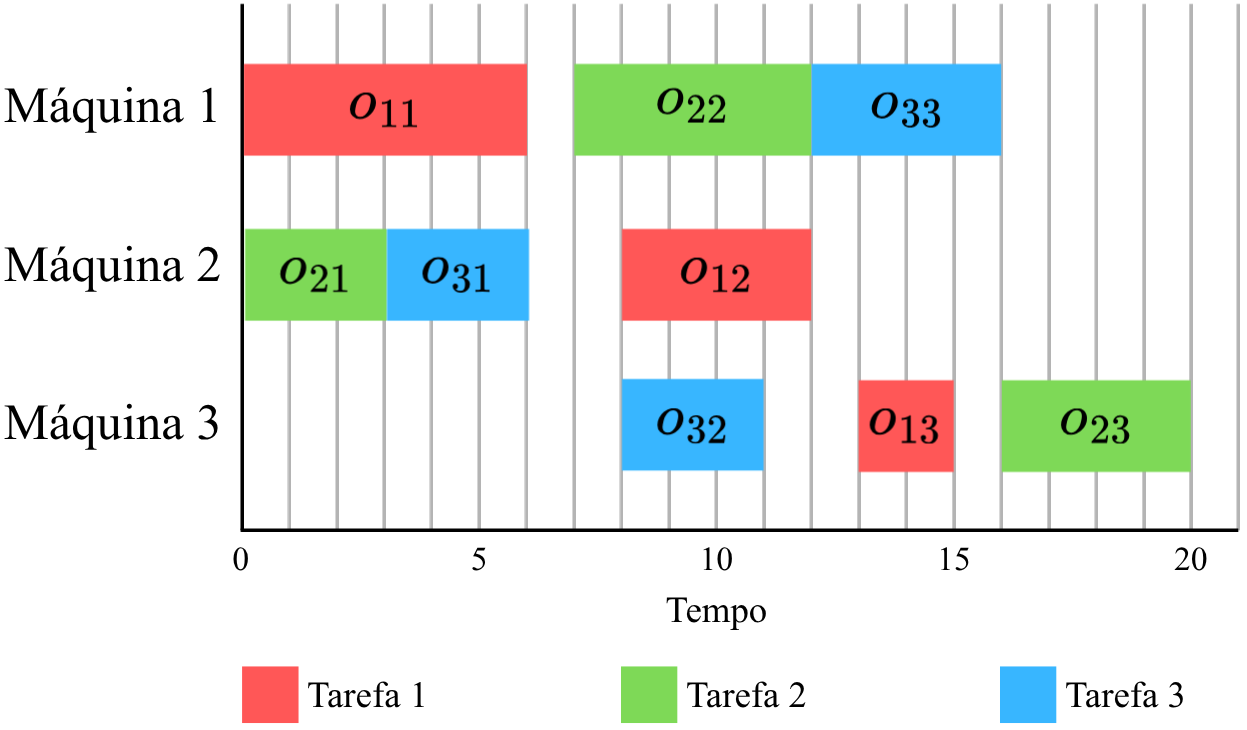
\includegraphics[width=0.75\linewidth]{img/exemplo_sol_jitjsp.png}
    \caption*{\small \textbf{Fonte:} Os Autores.}
\end{figure}

Dada a descrição e a modelagem do problema, podemos observar com mais detalhes o processo de encontrar uma solução para ele. Primeiramente, precisamos gerar uma sequência válida a partir da instância. Perceba que a instância do problema define uma ordem fixa para as operações de uma mesma tarefa, mas a ordem em que as operações utilizarão uma mesma máquina fica em aberto. Dessa forma, gerar uma sequência válida significa determinar a ordem de execução das operações em cada máquina. Para entender o processo de forma detalhada, precisamos introduzir o conceito de grafo disjuntivo na modelagem de problemas de agendamento.

\subsection{Grafo disjuntivo} \label{sect:grafo_disj}

Considere o grafo $G = (V, X, Y)$. Nesse grafo, para cada operação $o_{ik}$ de uma tarefa $J_i$, existe um vértice $u \in V$ representado por um par ordenado $(i,j)$, sendo $i$ o índice da tarefa e $j = M(o_{ik})$ o índice da máquina que processa essa operação. Além disso, o grafo possui dois conjuntos de arestas. As arestas conjuntivas $X$ e as arestas disjuntivas $Y$. As arestas conjuntivas são direcionadas e representam a ordem de processamento das operações de uma tarefa. Elas são dadas pela instância e existem apenas entre operações da mesma tarefa e, se a aresta $(u,v)$, $u,v \in V$, existe, a operação $u$ deve preceder a operação $v$. Enquanto isso, as arestas disjuntivas não são direcionadas e ligam operações que competem pela mesma máquina, isto é, se a aresta $\{u,v\}$, $u,v \in V$, existe, as operações $u$ e $v$ utilizam a mesma máquina. Adicionamos também dois vértices $s$ e $t$. O vértice $s$ possui $n$ arestas de saída na forma $(s,u)$ para cada vértice $u$ que representa a primeira operação de uma tarefa. Por outro lado, o vértice $t$ possui $n$ arestas de entrada na forma $(u,t)$ para cada vértice $u$ que representa a última operação de alguma tarefa. Definimos também uma função de pesos $w : V \to \mathbb{N}$ que mapeia cada vértice para um valor inteiro não negativo. Nesse âmbito, $w(s) = w(t) = 0$ \citep{pinedo2008}.

Considere novamente a instância do \ac{JITJSS} detalhada na Tabela \ref{tab:exemplo_agendamento}. A partir dessa instância, podemos gerar o grafo disjuntivo da Figura \ref{img:exemplo_grafo_disj}. Nessa figura, as arestas sólidas representam as arestas conjuntivas, enquanto as arestas tracejadas representam as arestas disjuntivas. De acordo com a definição do grafo disjuntivo para um problema de agendamento, podemos identificar as operações que utilizam uma mesma máquina. Na Figura em questão, os vértices em roxo representam as operações da máquina 1, os vértices em laranja representam a máquina 2 e os vértices em azul representam a máquina 3.

\begin{figure}[h!]
    \centering
    \caption{Grafo disjuntivo gerado a partir da instância de exemplo}
    \label{img:exemplo_grafo_disj}
    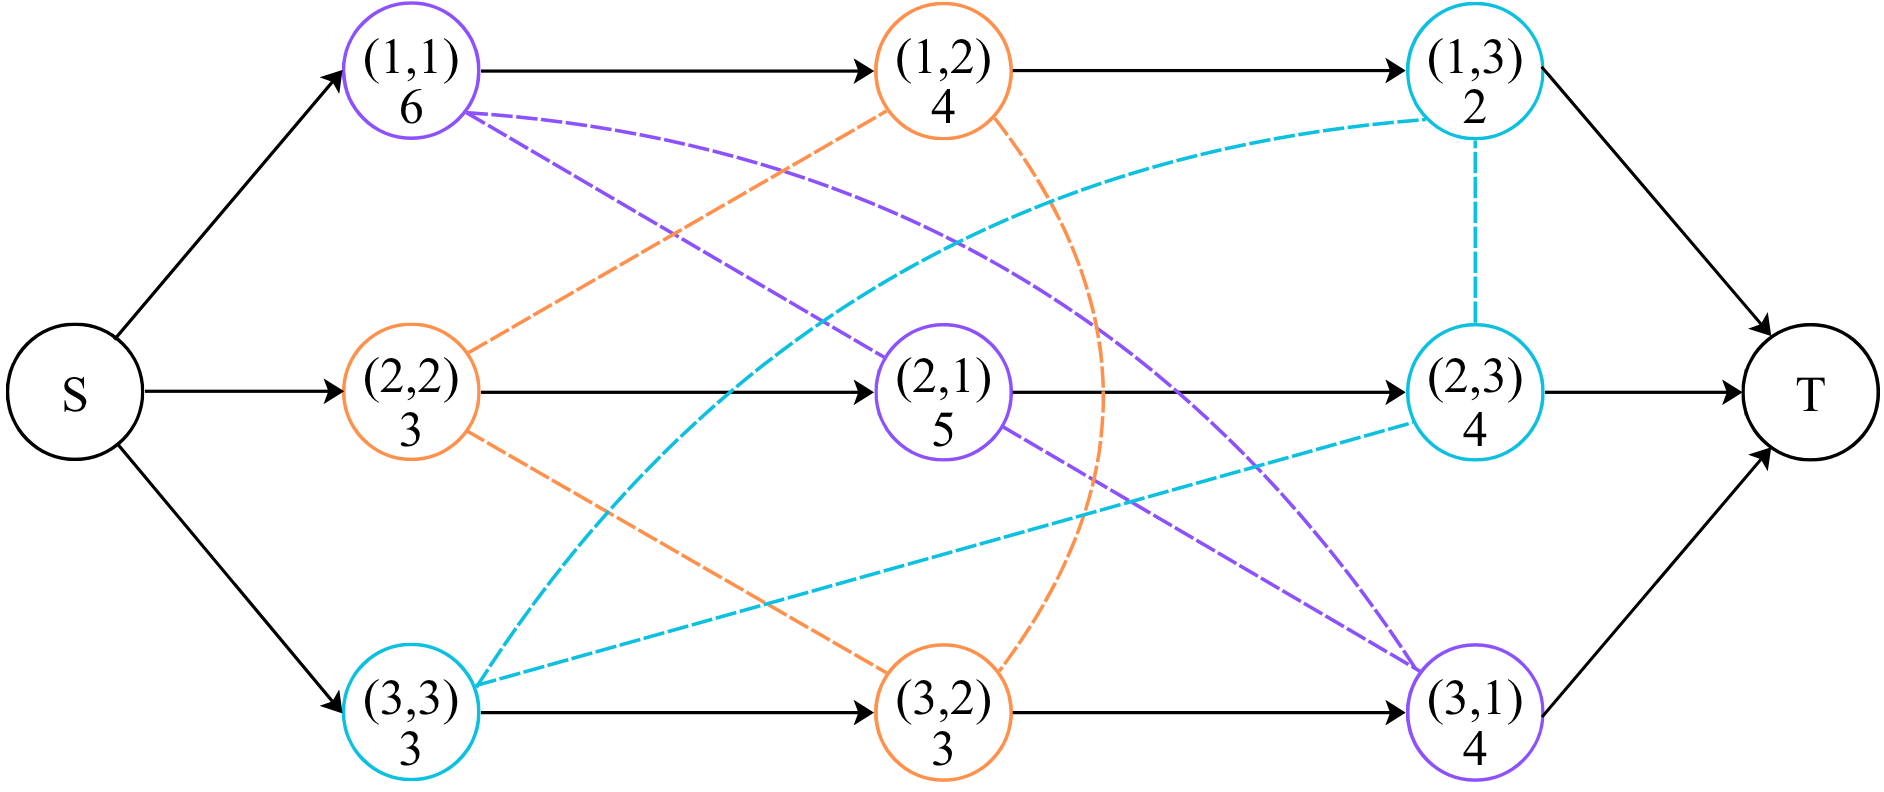
\includegraphics[width=0.75\linewidth]{img/grafo_disjuntivo.png}
    \caption*{\small \textbf{Fonte:} Os Autores.}
\end{figure}

Dessa forma, temos que, dada uma instância do problema, podemos gerar o grafo disjuntivo correspondente. Como mencionamos anteriormente, as arestas direcionadas do grafo disjuntivo implicam uma ordem de processamento das operações conectadas. Além disso, gerar uma sequência significa determinar a ordem de execução das operações em cada máquina. Por conseguinte, podemos definir que gerar uma sequência a partir de um grafo disjuntivo é o processo de selecionar direções para todas as arestas disjuntivas. Ao definir direções para todas as arestas disjuntivas, fazemos uma seleção completa e obtemos um grafo direcionado. Entretanto, para que a sequência seja viável, além da seleção completa, o grafo resultante precisa ser acíclico, pois um ciclo no grafo implicaria uma ordem de processamento impossível, na qual uma operação precederia a si mesma. Para a demonstração formal, veja \cite{pinedo2008}.


Podemos ver na Figura \ref{img:exemplo_dag} o mesmo grafo do exemplo anterior, mas com a seleção completa já aplicada. Dessa forma, observando o grafo, sabemos que a máquina 3 executará as operações $(3,3)$, $(1,3)$ e $(2,3)$ nessa ordem.

\begin{figure}[h!] 
    \centering
    \caption{Grafo direcionado acíclico que representa uma sequência viável}
    \label{img:exemplo_dag}
    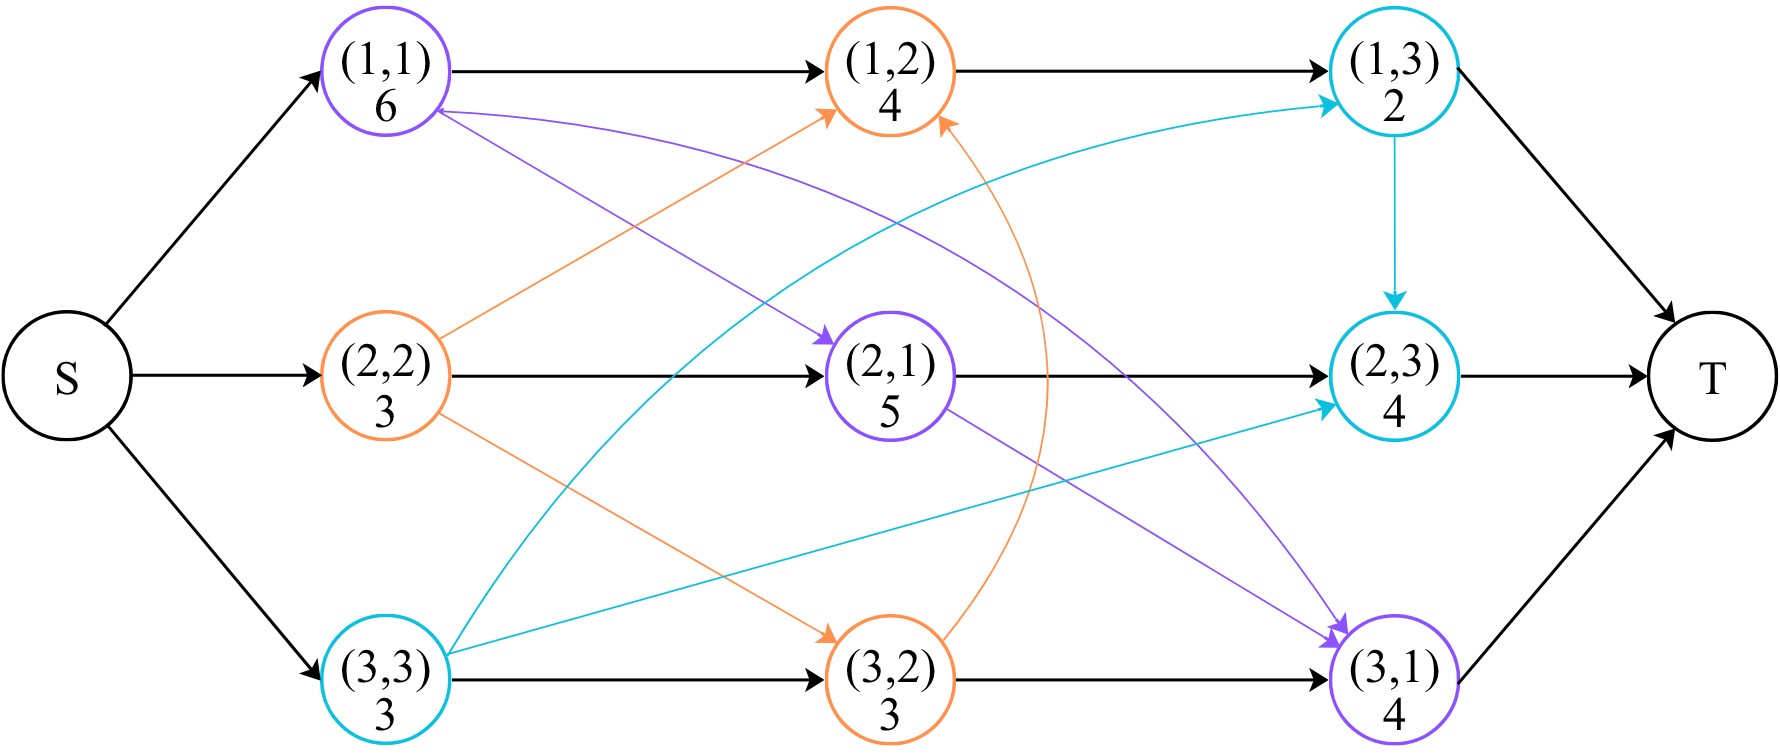
\includegraphics[width=0.75\linewidth]{img/grafo_selecao_completa.png}
    \caption*{\small \textbf{Fonte:} Os Autores.}
\end{figure}

Após encontrar uma sequência viável, precisamos avaliar a qualidade dessa sequência. Nesse sentido, uma das propriedades do grafo disjuntivo é que, após realizar a seleção das arestas disjuntivas, o caminho máximo do vértice $S$ ao $T$ é igual ao \textit{makespan} mínimo para essa seleção \citep{pinedo2008}. Por esse motivo, se nosso objetivo for minimizar o \textit{makespan}, dada uma sequência, podemos avaliar sua qualidade de forma ótima em tempo linear.

Por exemplo, o caminho máximo do grafo da Figura \ref{img:exemplo_dag} é composto pelos vértices $(1,1)$, $(1,2)$, $(1,3)$ e $(2,3)$, com peso total de 16. Podemos observar o agendamento que gera esse \textit{makespan} na Figura \ref{img:agendamento_makes}. O termo caminho crítico define esse percurso máximo, visto que as operações que o compõem impedem qualquer movimentação sem impacto no \textit{makespan}. Nesse sentido, nenhuma operação pertencente ao caminho crítico pode iniciar mais cedo sem que a sequência seja alterada.

Outra vantagem que temos ao minimizar o \textit{makespan}, sabendo o caminho crítico, é saber exatamente quais operações geram o \textit{makespan} de uma solução e, consequentemente, onde o agendamento exige modificações para alterar o \textit{makespan}. Essa informação auxilia o processo de minimização do \textit{makespan}, reduzindo o espaço de busca por melhorias.

\begin{figure}[h!] 
    \centering
    \caption{Agendamento ativo que minimiza o \textit{makespan}}
    \label{img:agendamento_makes}
    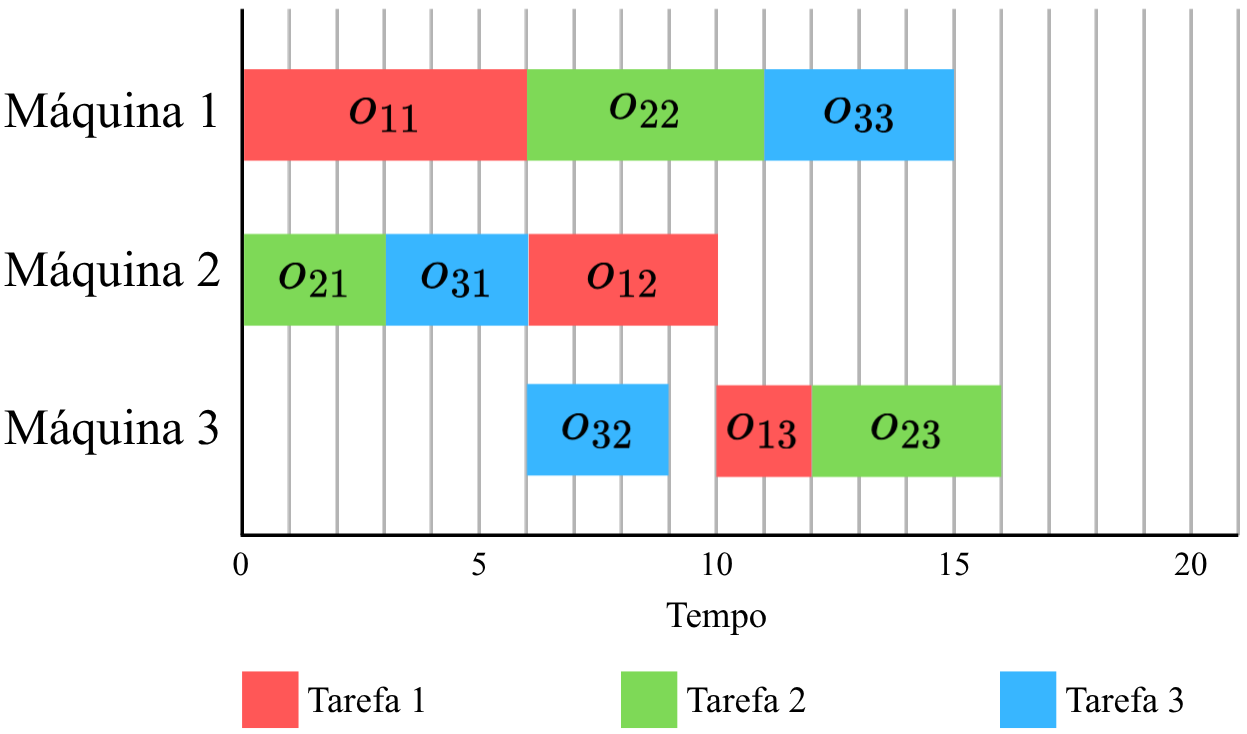
\includegraphics[width=0.75\linewidth]{img/agendamento_min_makes.png}
    \caption*{\small \textbf{Fonte:} Os Autores.}
\end{figure}

No entanto, se o nosso objetivo for minimizar as penalidades de adiantamento e atraso, não temos uma forma tão simples e rápida de gerar um agendamento ótimo a partir de uma sequência. O agendamento representado na Figura \ref{img:agendamento_makes} demonstra que agendar as operações o mais cedo possível não significa minimizar as penalidades, pois esse processo tende a gerar penalidades de adiantamento. Esse agendamento, por exemplo, gera uma penalidade total de 8,4, das quais 7,7 correspondem a penalidades por adiantamento. Ademais, poderíamos atrasar o início de algumas operações para que as penalidades fossem menores, o que nos levaria ao agendamento da Figura \ref{img:exemplo_sol_jitjsp}, que é ótimo para essa sequência específica. Veja a seção \ref{sect:bibjitjsp} para uma revisão bibliográfica que inclui as formas de gerar agendamentos utilizadas na literatura do \ac{JITJSS}.

\subsection{Algoritmos para geração de agendamentos} \label{sect:algs_constrs}

Nesta seção, apresentamos formas de gerar uma sequência viável por meio de exemplos de algoritmos. Nesse sentido, a literatura classifica procedimentos que constroem um agendamento do zero como construtivos. Estes algoritmos, de forma geral, precisam selecionar operação por operação a ser agendada até que todas sejam agendadas. Chamamos de regras de despacho as diferentes formas de selecionar qual operação agendar entre um conjunto de operações \citep{pinedo2008}. Tais algoritmos construtivos são capazes de utilizar qualquer regra de despacho internamente. Dessa forma, podemos definir um algoritmo que gera um agendamento baseado apenas em uma regra de despacho arbitrária.

Sejam, respectivamente, $J$, $M$ e $O$ os conjuntos de tarefas, máquinas e operações de um problema de agendamento. Dados esses conjuntos, definimos $o_{ik}$ como sendo a $k$-ésima operação da tarefa $i$. O algoritmo mantém uma lista $L$ de todas as operações para as quais todas as suas antecessoras já foram agendadas, isto é, se $o_{ik} \in L$, então as operações $o_{ix}$, nas quais $x < k$, já foram agendadas. O procedimento inicializa a lista $L$ com a primeira operação de cada tarefa e, a cada iteração, o algoritmo seleciona uma operação $o_{ik} \in L$ para ser agendada de acordo com uma regra de despacho e adiciona em $L$ a operação $o_{ik+1}$. Ao final de $|O|$ iterações, o algoritmo conclui o agendamento de todas as operações em $O$ \citep{pinedo2008}.

Outro algoritmo um pouco mais sofisticado é o \ac{GT} \citep{giffler1960algorithms} para geração de agendamentos ativos. Um agendamento é ativo quando não é possível alterar a posição de uma operação no agendamento para que ela inicie mais cedo sem que um atraso em outra operação seja causado, em outras palavras, o agendamento não possui tempo ocioso entre duas operações no qual fosse possível agendar outra operação. Por exemplo, o agendamento da Figura \ref{img:agendamento_makes} é um agendamento ativo. O algoritmo \ac{GT} utiliza as mesmas estruturas que o algoritmo descrito anteriormente, mas, antes de utilizar uma regra de despacho para selecionar uma operação, ele realiza filtros na lista $L$ para que apenas operações que mantém o agendamento ativo sejam escolhidas.

Seja $P(o_{ik}) \in \mathbb{N}$ o tempo de processamento da operação $o_{ik}$ e $A(o_{ik}) \in O$ a operação que antecede $o_{ik}$ na mesma máquina. Definimos o tempo de término de uma operação $C(o_{ik}) = max(C(o_{ik-1}), C(A(o_{ik})) + P(o_{ik})$. O algoritmo \ac{GT} seleciona em $L$ a operação $o'$ com menor tempo de término $C'$. A partir dessa operação, o algoritmo cria a lista $L_1 \subseteq L$ que contém as operações $o''$ as quais $M(o'') = M(o')$ e $C(o'') \le C'$. O algoritmo, então, aplica uma regra de despacho na lista $L_1$ para selecionar a operação $o_{ik}$ que será agendada, remove $o_{ik}$ de $L$ e adiciona $o_{ik+1}$ em $L$ se $o_{ik+1} \in O$. Após $|O|$ iterações, o algoritmo produz um agendamento viável e ativo.

\section{Configuração Automática de Algoritmos}

No processo de desenvolver estratégias de resolução para problemas inerentemente difíceis como o \ac{JITJSS}, uma das alternativas que possuímos é utilizar heurísticas. Uma heurística resolve o problema em tempo viável, mas não garante a qualidade das soluções que encontra, no sentido de que não é possível demonstrarmos que as soluções são ótimas ou que possuem algum limite de aproximação da solução ótima \citep{talbi}.

Durante o desenvolvimento dessas estratégias, os pesquisadores perceberam que grupos de diferentes heurísticas para problemas diferentes possuem diversas características em comum. Por exemplo, toda heurística de busca possui algum tipo de construção, recombinação ou modificação de soluções dentro do seu processo de exploração do espaço de busca. Esses conceitos são independentes de características específicas de cada problema. Por outro lado, ao observarmos a aplicação desses conceitos na literatura, percebemos estratégias específicas que os autores implementam para servir às peculiaridades do problema-alvo \citep{zbb}.

A partir dessas ideias, abstraímos os conceitos comuns entre diferentes estratégias e definimos métodos que podemos aplicar em qualquer problema, mas que possuem lacunas que devemos preencher com os componentes específicos ao problema que estamos resolvendo. A comunidade científica chama esses métodos genéricos de meta-heurísticas \citep{zbb}.

O desenvolvimento de meta-heurísticas eficientes em resolver um problema leva tempo e exige do projetista um conhecimento profundo das características do problema. As meta-heurísticas tendem a facilitar esse processo por meio da generalização de métodos em comum que funcionaram para diferentes problemas. Ainda assim, desenvolver uma meta-heurística eficiente é um processo custoso. Nessa perspectiva, os projetistas de meta-heurísticas precisam tomar diversas decisões de projeto, tanto de alto quanto de baixo nível. Esses projetistas podem basear essas decisões em testes exaustivos, buscando encontrar uma configuração que retorne os melhores resultados. Porém, essa abordagem é tediosa, propensa a erros e dificilmente reproduzível \citep{birattari2009tuning}.

Com o avanço e maior disponibilidade do poder computacional e visando mitigar o problema de configurar heurísticas, a comunidade científica propôs diversos métodos de \ac{AAC}. Dessa forma, os pesquisadores podem executar o trabalho repetitivo e tedioso automaticamente, ganhando tempo para, por exemplo, desenvolver novas estratégias para a resolução de problemas \citep{birattari2009tuning}.

Esta seção aborda a \ac{AAC} como um problema de otimização e as principais ferramentas para resolvê-lo, detalhando inicialmente os conceitos fundamentais de vizinhanças e meta-heurísticas. No entanto, considerando o objetivo do presente trabalho, não realizaremos uma revisão abrangente de todos os tipos de meta-heurísticas, mas detalharemos apenas aquelas relacionadas ao domínio do projeto. Dessa forma, para detalhes e definições sobre meta-heurísticas, nos referimos aos trabalhos de \cite{talbi} e \cite{zbb}.

% Esta seção aborda conceitos de configuração automática. Primeiro, ela define conceitos fundamentais de meta-heurísticas e explica as meta-heurísticas mais importantes para o presente trabalho. Em seguida, explica a configuração automática enquanto um problema de otimização e apresenta as principais ferramentas utilizadas no processo de configuração automática. Muitas estratégias heurísticas citadas ao longo do trabalho não serão completamente detalhadas. Dessa forma, para detalhes e definições de cada meta-heurística citada no restante deste trabalho, veja .

\subsection{Vizinhanças}

Dado o conjunto de todas as soluções $S$ de um problema, \cite{talbi} define uma vizinhança como um mapeamento de cada solução $s \in S$ para um subconjunto de soluções $N(s) \subseteq S$. Chamamos de vizinha de $s$ uma solução $s' \in N(s)$. O mapeamento da vizinhança modifica soluções sistematicamente para gerar novas soluções. Por isso, a vizinhança é uma componente específica do problema-alvo, isto é, sua forma e eficiência dependem exclusivamente das características do problema. Isso é verdade, pois modificar uma solução inclui manipular a representação da solução, que varia entre problemas e até mesmo entre diferentes abordagens sobre o mesmo problema \citep{talbi}.

O projetista de uma vizinhança deve considerar algumas características durante o desenvolvimento. Uma delas é a localidade da vizinhança; essa propriedade consiste no impacto que alterações na representação de uma solução têm sobre a qualidade da solução. Se pequenas alterações na representação causam pequenas mudanças na solução, a vizinhança possui alta localidade. Por outro lado, se pequenas alterações na representação causam grandes mudanças na solução, a vizinhança possui baixa localidade. Diante disso, uma exploração do espaço de busca por meio de uma vizinhança com alta localidade é mais refinada e sistemática \citep{talbi}.

Outro ponto importante é o tamanho da vizinhança. Gerar e explorar uma vizinhança muito grande pode ter um custo alto e, consequentemente, atrapalhar o processo de busca. Por outro lado, vizinhanças muito restritas e, consequentemente, pequenas, podem ignorar soluções promissoras no espaço de soluções. \citep{talbi}.

Com o conceito de vizinhança estabelecido, podemos introduzir o conceito de ótimo local. Esse conceito é importante pois diversas meta-heurísticas mais sofisticadas implementam múltiplas técnicas para evitar ótimos locais. \cite{talbi} define um ótimo local como uma solução $s'$ tal que, para toda solução vizinha $s'' \in N(s')$, temos que $f(s') \leq f(s'')$. Um ótimo global, por sua vez, é uma solução $s'$ que, para qualquer solução $s''$ do espaço de busca, $f(s') \leq f(s'')$ \citep{talbi}. Note que, por definição, todo ótimo global é também um ótimo local, mas o inverso não é verdadeiro. A Figura \ref{img:exemplo_minimos_locais} apresenta um gráfico que representa os valores de $f$ pelo espaço de busca e indica os ótimos locais e um ótimo global.

\begin{figure}[h!] 
    \centering
    \caption{Mínimos locais em relação à função objetivo no espaço de soluções}
    \label{img:exemplo_minimos_locais}
    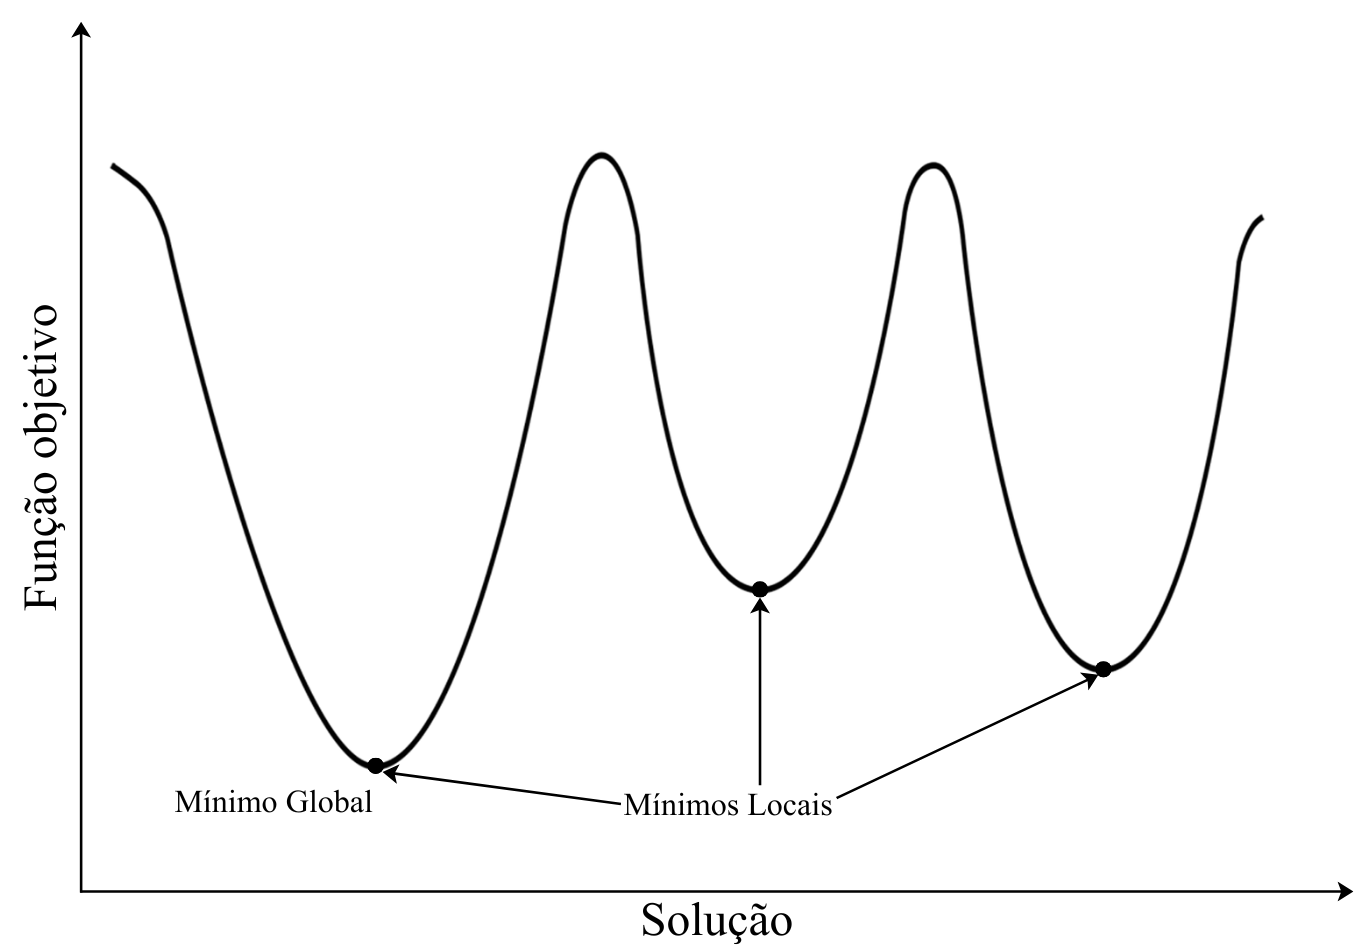
\includegraphics[width=0.75\linewidth]{img/minimos_locais.png}
    \caption*{\small \textbf{Fonte:} Adaptado de \cite{talbi}}
\end{figure}

\subsection{Meta-heurísticas} \label{sect:meta}

Como mencionamos anteriormente, as meta-heurísticas são estratégias de alto nível que podemos aplicar a qualquer problema. Em vista disso, a Busca Local (do inglês, Local
Search -- \acs{LS}) é uma das meta-heurísticas mais básicas e, por isso, as meta-heurísticas mais sofisticadas utilizam seus conceitos internamente. Dada uma solução inicial $s_0$, a cada iteração $i$, a busca local gera a vizinhança $N(s_i)$ da solução $s_i$. Assim, a busca local seleciona uma solução $s_{i+1} \in N(s_i)$ tal que $f(s_{i+1}) < f(s_i)$, em outras palavras, seleciona uma solução que melhora a função objetivo. Por fim, o algoritmo finaliza o processo de busca quando não existe nenhuma solução $s' \in N(s_i)$ de forma que $f(s') < f(s_i)$. Por esse motivo, a busca local não consegue escapar de ótimos locais no espaço de busca \citep{talbi}.

Podemos realizar a exploração do espaço de busca e a seleção de vizinhos na busca local de diferentes formas. Uma delas, a seleção por melhor melhora, consiste em selecionar o melhor vizinho de uma solução a cada iteração, isto é, tendo uma solução $s_i$, o algoritmo seleciona a vizinha de $s_i$ que oferece o máximo de melhoria na função objetivo em relação a $f(s_i)$. Utilizar esse tipo de seleção significa gerar e avaliar todos os vizinhos da solução a cada iteração. Esse processo pode ter um custo elevado em vizinhanças grandes \citep{talbi}.

Outra forma de selecionar vizinhos consiste em selecionar o primeiro vizinho de $s_i$ que melhora a função objetivo. Por isso, ao contrário da primeira opção, o algoritmo não precisa gerar nem avaliar toda a vizinhança. Isso gera uma exploração do espaço de busca mais rápida; porém, corremos o risco de que o processo ignore boas soluções simplesmente pela ordem de geração e avaliação dos vizinhos. Chamamos essa segunda estratégia de seleção por primeira melhora \citep{talbi}.

O maior problema de uma busca local simples é a incapacidade de escapar de ótimos locais. Por esse motivo, buscas locais tendem a finalizar o processo de busca precocemente e sem realizar uma exploração satisfatória no espaço de busca. Com isso em mente, apresentamos o conceito de perturbação de uma solução. Meta-heurísticas mais complexas utilizam esse processo com o objetivo de escapar de ótimos locais. Ele geralmente se aplica aos ótimos locais e consiste em realizar alguma modificação da solução que seja significativa o suficiente para que a solução modificada se afaste do ótimo local \citep{talbi}. Por exemplo, no gráfico da Figura \ref{img:exemplo_perturbacao}, temos duas funções de perturbação, $g'$ e $g''$. Nesse caso da imagem, a função $g'$ não fez uma perturbação efetiva, pois a solução gerada não é diferente o suficiente para gerar um mínimo local diferente. Por outro lado, a função $g''$ gera uma solução que levará o processo de busca a um mínimo local diferente e melhor.

\begin{figure}[h!] 
    \centering
    \caption{Transformações de mínimos locais por funções de perturbação.}
    \label{img:exemplo_perturbacao}
    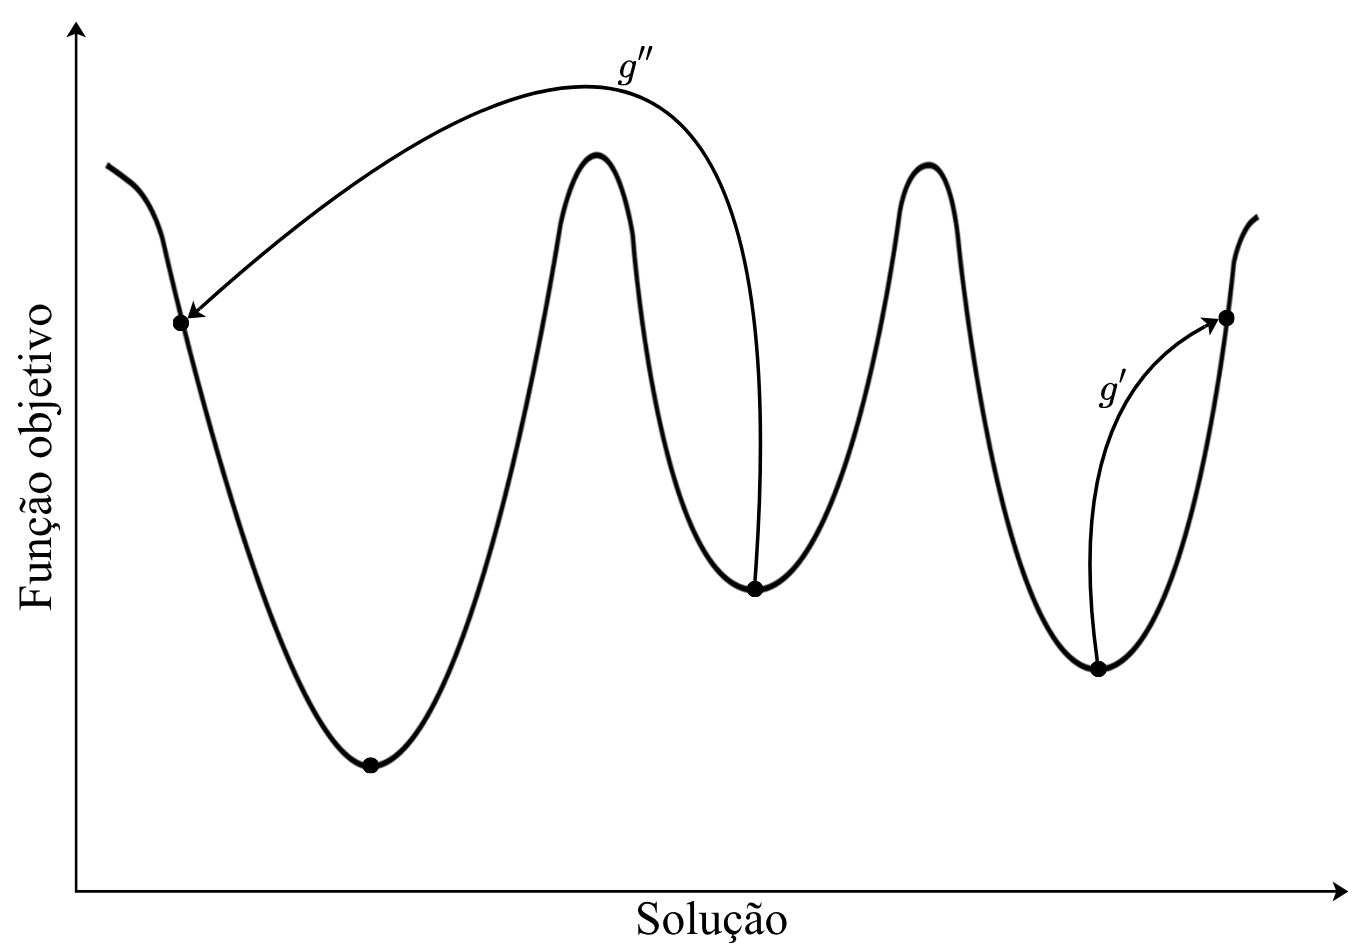
\includegraphics[width=0.75\linewidth]{img/exemplo_perturbacao.png}
    \caption*{\small \textbf{Fonte:} Os Autores.}
\end{figure}

A Busca Local Iterada (do inglês, Iterated Local
Search -- \acs{ILS}) é um exemplo de meta-heurística que utiliza um processo de perturbação em seu processo de busca. Ela realiza, iterativamente, buscas locais com diferentes soluções iniciais para encontrar diferentes ótimos locais. Em cada iteração, ela utiliza uma perturbação do ótimo local encontrado na iteração anterior \citep{talbi}. Algumas características da \ac{ILS} incluem a possibilidade de utilizar qualquer heurística de solução única como método de busca, isto é, o processo de encontrar um ótimo local a cada iteração é uma caixa-preta. Nesse sentido, essa caixa-preta deve receber uma solução e encontrar um ótimo local \citep{talbi}.

Algumas meta-heurísticas renomeiam o processo de perturbação. Por exemplo, a Busca em Vizinhança Variável (do inglês, Variable Neighborhood Search -- \acs{VNS}) chama esse processo de \textit{shake}. Essa meta-heurística se apoia na ideia de que diferentes vizinhanças de um mesmo problema exploram subespaços de busca diferentes. Mais especificamente, podemos dividir o processo de busca na \ac{VNS} em três fases: \textit{Shake}, busca local e \textit{move}. Dada uma lista de estruturas de vizinhança $N = \{N_1, N_2,...N_{n-1}, N_n\}$, a cada iteração, a \ac{VNS} realiza o \textit{shake} de uma solução inicial $s$ pela vizinhança atual $N_k \in N$, isto é, o algoritmo seleciona uma solução $s'$ aleatoriamente da vizinhança $N_k(s)$. Após o \textit{shake}, a \ac{VNS} aplica um processo de busca local sobre a solução $s'$, encontrando um ótimo local $s''$. Por fim, caso $f(s'') < f(s)$, a \ac{VNS} realiza o \textit{move}, ou seja, seleciona $s''$ como a nova solução base e redefine $k=1$; caso contrário, mantém a solução e incrementa $k$, $k = k+1$ \citep{talbi}.

% Por fim, apesar de não garantirem a qualidade das soluções obtidas, as meta-heurísticas se provaram excelentes opções para resolver problemas. Por exemplo, o estado da arte para o \ac{JITJSS} é composto majoritariamente por meta-heurísticas como os algoritmos \ac{VNS} de \cite{ahmadian2021meta} e \cite{wang2014variable}, a busca adaptativa em grandes vizinhanças de \cite{abderrazzak2022adaptive} e o algoritmo evolucionário de \cite{dos2010combination}.

Dando continuidade às estratégias de evasão de mínimos locais, também podemos utilizar a Busca Tabu (do inglês, \textit{Tabu Search} -- \acs{TS}). Essa meta-heurística é semelhante à busca local no sentido de que inicia a busca a partir de uma solução inicial $s_0$ e explora o espaço de busca iterativamente, selecionando novas soluções que melhoram a função objetivo. Porém, a busca tabu não encerra a busca ao chegar a um ótimo local no espaço de busca. Ao invés disso, a busca seleciona uma solução que piora a função objetivo para escapar do ótimo local. Nesse sentido, ela seleciona o vizinho com o menor valor da função objetivo, mesmo que ele não seja melhor que a solução que o gerou \citep{talbi}.

% Durante a exploração do espaço de soluções na busca local, a solução da iteração atual é sempre melhor que todas as soluções de iterações anteriores. Por outro lado,
Ao selecionar soluções que pioram a função objetivo, a busca tabu permite que soluções selecionadas em iterações anteriores sejam melhores que a solução da iteração atual. Por isso, é intuitivo pensar que a busca pode ficar presa em um ciclo infinito de pioras e melhoras da função objetivo. Porém, a busca tabu utiliza uma memória para evitar selecionar soluções repetidas. Ela implementa essa memória em uma lista tabu de movimentos realizados, e não seleciona novas soluções que desfazem esses movimentos tabu. É importante mencionar que a lista tabu mantém os estados da busca por um período denominado $tenure$ \citep{talbi}.

% A implementação da lista tabu depende de características específicas do problema-alvo. Armazenar as soluções integralmente nem sempre é viável pelo espaço de armazenamento necessário e pelo custo de verificar se uma solução está na lista. Por isso, em certos problemas, é mais vantajoso armazenar uma informação parcial das soluções e, com isso, ganhar eficiência de verificação da lista em detrimento da precisão de verificação \citep{talbi}.
% Por exemplo, podemos implementar a lista tabu de forma que ela armazene os movimentos que o algoritmo realizou na solução entre cada iteração e barrar novas soluções que revertam esses movimentos. Essa estratégia torna eficiente verificar se a lista tabu permite um movimento, mas não impede que o algoritmo selecione soluções repetidas, visto que, em certos problemas, é possível retornar à mesma solução por diferentes sequências de modificações \citep{talbi}.  

A implementação ideal de uma meta-heurística sobre um problema deveria obter bons resultados em todos os tipos diferentes de instâncias do problema. Porém, construir soluções que atinjam essa generalização de forma completa nem sempre é possível \citep{birattari2009tuning}. Por exemplo, suponha um algoritmo de busca local para um certo problema $X$, talvez a seleção por primeira melhora seja a melhor opção para um determinado grupo de instâncias, mas, para um grupo diferente de instâncias, a seleção por melhor melhora seja ideal. O projetista precisa escolher qual tipo de seleção implementar, ou por primeira melhora, ou por melhor melhora, ou até mesmo por uma terceira forma híbrida. Esse tipo de decisão se repete constantemente no desenvolvimento de soluções. Nesses casos, o projetista pode definir e implementar uma das opções ou implementar todas e permitir ao usuário do algoritmo escolher a abordagem por meio de um parâmetro. Dessa forma, o usuário pode decidir as estratégias mais adequadas aos tipos de instâncias em questão \citep{birattari2009tuning}.

Definir parâmetros customizáveis parece resolver o problema, pois gera algoritmos mais flexíveis. Porém, mesmo assim, o projetista ainda precisou realizar uma série de decisões que compõem a base desse algoritmo flexível. Além disso, o usuário também precisará definir uma série de parâmetros de acordo com suas necessidades. Diante disso, uma das alternativas para tomar tais decisões é realizar múltiplos testes até encontrar uma configuração razoável. Porém, essa abordagem tem alguns problemas \citep{birattari2009tuning}.

Primeiramente, para que esse processo seja efetivo, o indivíduo que configurar o algoritmo precisa ter um conhecimento profundo do problema em questão, além de conhecer detalhadamente o algoritmo em si. Além disso, esse tipo de configuração pode invalidar completamente os resultados da comparação entre algoritmos. Por exemplo, considere que um projetista comparou dois algoritmos $A$ e $B$. Nesse processo, ele passou 75\% do seu tempo configurando o algoritmo $A$ e os outros 25\% configurando o $B$. Independentemente de qual algoritmo obteve os melhores resultados, o viés da configuração invalida a comparação. Ou seja, os resultados dependem da imparcialidade do projetista que configurou os algoritmos \citep{birattari2009tuning}.

É nesse contexto que surge a necessidade de métodos científicos e formais para configurar algoritmos. 

% Pois, dado que um ótimo local possui características de uma boa solução, pode ser mais vantajoso continuar a busca a partir dos seus vizinhos ao invés de voltar para uma solução aleatória \citep{talbi}.
% Essa estratégia é baseada na ideia de que, sendo o ótimo local a melhor solução em uma certa área do espaço de busca, ele possui características de uma boa solução e, por isso, devemos manter algumas delas para alcançar outra boa solução \citep{talbi}.

% Além disso, o processo de perturbação do ótimo local é outro componente importante para a \ac{ILS}. Esse procedimento tem como objetivo afastar o processo de busca dos ótimos locais encontrados em cada iteração. O impacto da perturbação na solução pode variar a depender da estratégia. Por exemplo, quando o processo de busca utilizado é altamente eficiente, realizar uma pequena modificação na solução fará com que o processo de busca encontre o mesmo ótimo local na próxima iteração, fazendo a \ac{ILS} ficar presa em um ciclo \citep{talbi}.

% Por fim, após realizar a perturbação e o processo de busca sobre o ótimo local perturbado, a \ac{ILS} utiliza, na próxima iteração, o novo ótimo local encontrado pela heurística de busca apenas se ele passar em um critério pré-determinado. Esse critério varia em um espectro no qual um dos extremos é aceitar apenas soluções que melhoram a função objetivo e o outro extremo é aceitar soluções independentemente de seus valores na função objetivo. Ao utilizarmos uma \ac{ILS} para resolver um problema, é importante encontrarmos um ponto nesse espectro que seja adequado às particularidades do problema-alvo \citep{talbi}. 

\subsection{Problema de Configuração \textit{offline} de algoritmos}

Dado o contexto de utilização da \ac{AAC}, podemos definir a configuração de algoritmos como um problema de otimização. Perceba que o objetivo da configuração de algoritmos é, dado um algoritmo e instâncias de um problema, determinar os parâmetros do algoritmo que maximizam sua performance nessas instâncias \citep{birattari2009tuning}. Nesta subseção, formalizaremos esse problema.

Chamamos o problema de \textit{offline} pela forma como ele realiza a otimização da configuração. Em métodos \textit{offline}, a busca no espaço de configurações ocorre em uma fase de treinamento e a melhor configuração encontrada é, então, utilizada em produção. Usualmente, utilizamos um conjunto de instâncias de treinamento e, como forma de validar as configurações obtidas, utilizamos um conjunto diferente de instâncias para testar essas configurações obtidas \citep{birattari2009tuning}.

Definimos aqui o problema de configuração de algoritmos. Seja $\mathcal{A}$ um algoritmo com $n$ parâmetros $p_i$ e $1 \leq i \leq n$, de forma que cada parâmetro $p_i$ possua domínio $\Theta_i$. Temos que o espaço de configurações $\Theta \subseteq \Theta_1 \times \Theta_2 \times \ldots \times \Theta_n$ contém todas as combinações de parâmetros válidas do algoritmo $\mathcal{A}$. Dessa maneira, dado um conjunto de instâncias $\Pi$ e uma função de custo $c(\theta, \pi)$ que mede o custo de executar $\mathcal{A}$ sobre a instância $\pi \in \Pi$ com uma configuração $\theta \in \Theta$, o objetivo do problema é encontrar uma configuração $\theta^* \in \Theta$ que minimize o custo de $\mathcal{A}$ sobre todo o conjunto $\Pi$. Podemos ver essa função objetivo na Equação \ref{eq:2.9}, onde $\mathcal{C}$ é uma função agregada de $c(\theta, \pi)$ sobre todas as instâncias $\pi \in \Pi$ \citep{souza2022automatic}.

\begin{align} \label{eq:2.9}
&\theta^* \in \operatorname{argmin}\mathcal{C}(\theta, \Pi) &&\theta \in \Theta
\end{align}

Podemos utilizar como função agregada $\mathcal{C}$, a exemplo, o desempenho médio em todas as instâncias $\mathcal{C}(\theta, \Pi) = \sum_{\pi \in \Pi} c(\theta, \pi) / |\Pi|$ ou o pior desempenho encontrado em qualquer uma das instâncias $\mathcal{C}(\theta, \Pi) = \max_{\pi \in \Pi} c(\theta, \pi)$.

Um algoritmo parametrizado pode ter parâmetros de diferentes tipos. Nesse sentido, parâmetros categóricos definem um conjunto fixo de opções para o algoritmo. Utilizamos esse tipo de parâmetro frequentemente para definir estratégias do algoritmo para atingir um mesmo fim, por exemplo, qual vizinhança utilizar em uma busca local. Os parâmetros também podem ser ordinais, isto é, seus valores possuem uma relação de ordem intrínseca. Por exemplo, considere o mesmo parâmetro de escolha de vizinhança em uma busca local, mas, agora, as vizinhanças estão ordenadas pelo seu tamanho. Por fim, também temos os parâmetros numéricos. Eles mapeiam valores inteiros ou reais do algoritmo, como, por exemplo, constantes utilizadas em cálculos e funções, ou a temperatura inicial de um algoritmo de Recozimento Simulado (do inglês, \textit{Simulated Annealing} - \acs{SA}) \citep{lopez2016irace}.

Além dos diferentes tipos, podemos definir relações entre parâmetros. Uma relação condicional acontece quando um parâmetro pode ser definido apenas se outro parâmetro também for definido. Por exemplo, em um algoritmo que utiliza diferentes meta-heurísticas definidas por um parâmetro, só faz sentido definir o parâmetro \textit{tenure} se o algoritmo alvo utilizar a meta-heurística Busca Tabu. Parâmetros também podem impor restrições a outros parâmetros. Por exemplo, em um algoritmo evolutivo, o número de indivíduos selecionados para o processo de \textit{crossover} não pode ser maior do que o tamanho da população. Por fim, algumas combinações de parâmetros não são permitidas, pois podem causar erros ou comportamentos indefinidos no algoritmo \citep{lopez2016irace}.

Assim, podemos definir uma instância do problema de configuração de algoritmos. Ela é uma sêxtupla $I=(\mathcal{A}, \Theta, \Pi, c , B, S)$ onde $\mathcal{A}$ é o algoritmo alvo da configuração, $\Theta$ é o espaço de configurações, $\Pi$ é um conjunto de instâncias de treinamento, $c$ é uma métrica de custo, $B$ é a quantidade de recursos disponíveis para configuração e $S$ é um conjunto de informações adicionais \citep{hutter2009paramils}. Mais especificamente, o recurso $B$ diz respeito ao recurso computacional disponível para realizar essa configuração e, usualmente, medimos em iterações ou em tempo de processamento. Além disso, também temos as configurações adicionais $S$ que incluem, por exemplo, fatores relacionados ao processo de configuração, a alguma configuração do algoritmo ou às instâncias de teste. Por exemplo, o conjunto $S$ pode conter configurações iniciais para o configurador, o critério de parada do algoritmo ou argumentos específicos para certas instâncias.

Mesmo com o problema formalizado, precisamos de maneiras de resolvê-lo. Uma abordagem possível seria fazer isso manualmente através de testes e observação das melhores configurações. Porém, como já mencionamos, esse tipo de processo ocupa muito tempo dos projetistas de algoritmos, principalmente para testar configurações ruins. Além disso, o processo é muito difícil de replicar e pode gerar configurações enviesadas que, consequentemente, produzem resultados inválidos. Por esses motivos, precisamos de métodos sistemáticos para resolver o problema da configuração de algoritmos \citep{birattari2009tuning}

\subsection{Processo de configuração automática e configuradores} \label{sect:ref_conf_auto_configuradores}

O processo de \ac{AAC} consiste em utilizar os recursos computacionais disponíveis para explorar o espaço de configurações. Chamamos a ferramenta que realiza essa exploração de configurador. Na Figura \ref{img:diagrama_configurador} podemos observar a organização e o fluxo dos componentes de um configurador. O algoritmo configurador recebe como entrada a instância definida na subseção anterior. A partir disso, ele realiza chamadas do algoritmo $\mathcal{A}$ sobre uma determinada instância $\pi$ com a configuração $\theta$. O algoritmo $\mathcal{A}$, então, retorna o valor da métrica $c$ para a instância e configuração fornecidas. Dessa maneira, o configurador avalia configurações e explora o espaço de busca sistematicamente. Ao consumir todo o recurso computacional $B$, o configurador retorna a configuração (ou configurações) que teve o melhor desempenho agregado nas instâncias de treinamento. \citep{hutter2009paramils}.

\begin{figure}[h!] 
    \centering
    \caption{Fluxo de execução de um algoritmo configurador}
    \label{img:diagrama_configurador}
    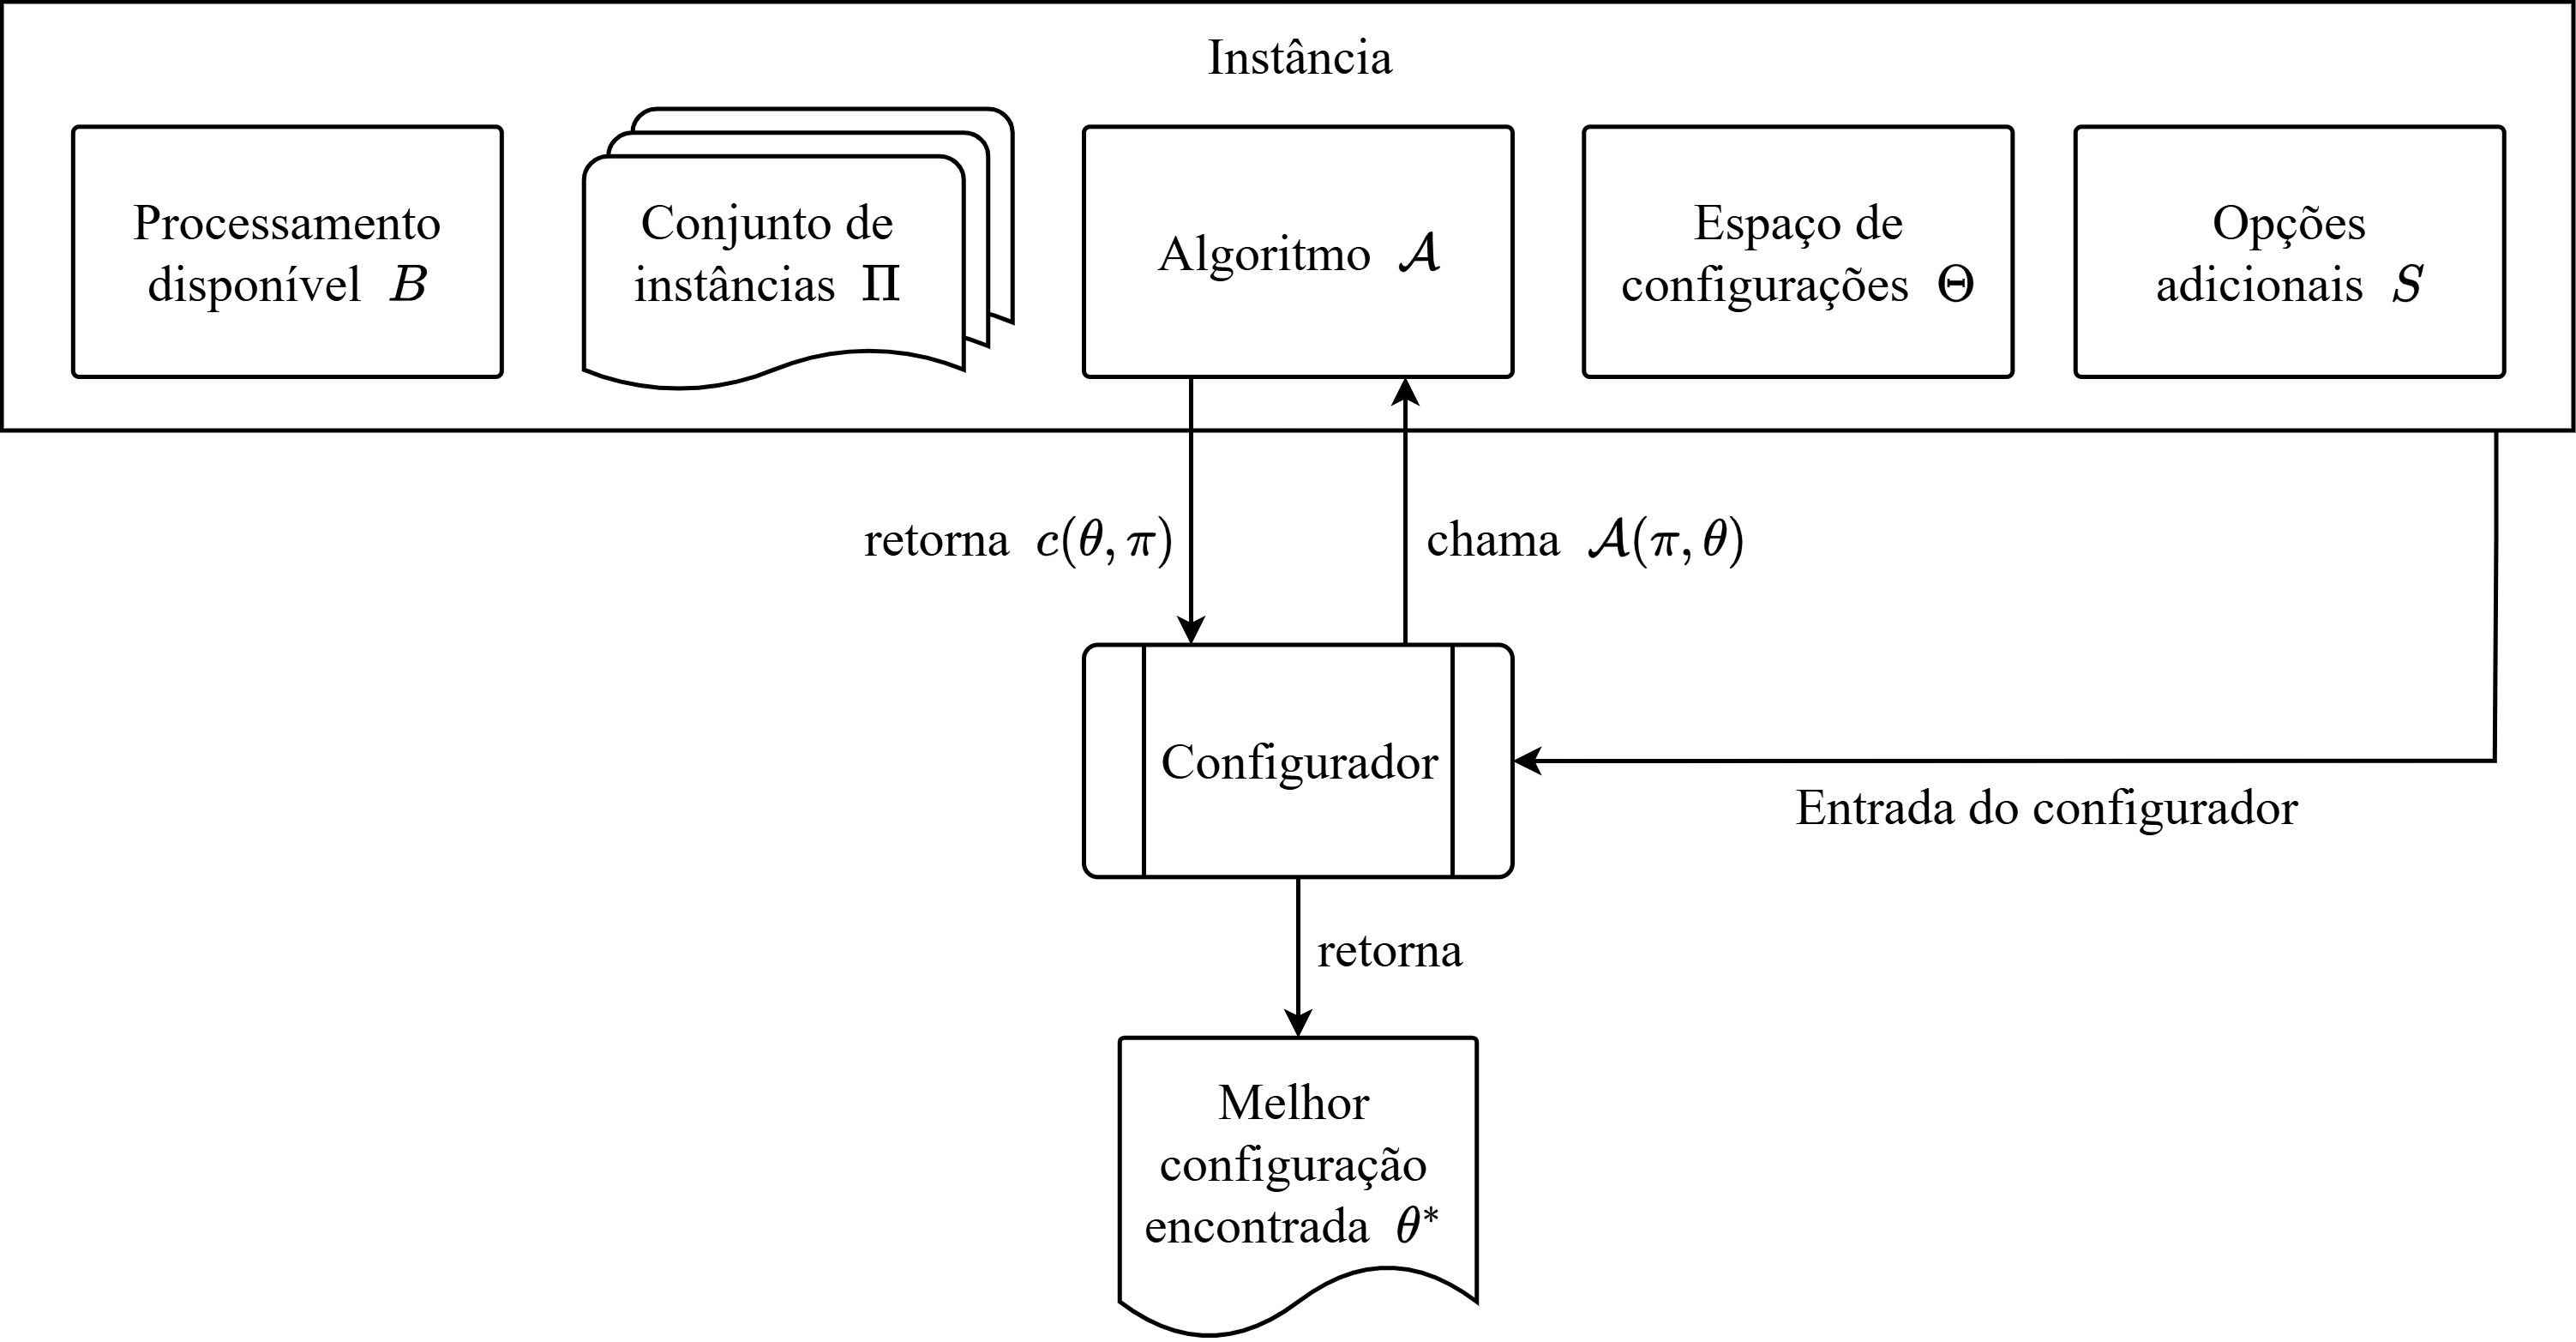
\includegraphics[width=0.85\linewidth]{img/diagrama_configurador.png}
    \caption*{\small \textbf{Fonte:} Adaptado de \cite{souza2022automatic}}
\end{figure}

O processo de \ac{AAC} é desafiador por diversos motivos. O trabalho de \cite{souza2022automatic} organiza esses desafios, identificados durante o desenvolvimento dos diversos configuradores da literatura. Um dos desafios a superar é a dificuldade de obter um conjunto de configurações que otimize a função objetivo para todas as instâncias de treinamento. O configurador precisa avaliar corretamente as métricas de qualidade independentemente da instância para que ele explore corretamente o espaço de soluções. Por exemplo, instâncias com custos de escalas diferentes não podem enviesar o configurador, fazendo-o focar apenas na otimização da instância de maior magnitude.

Outro desafio é a natureza estocástica de certos algoritmos. Nesses casos, podemos precisar de múltiplas execuções do algoritmo alvo para obter uma informação relevante sobre a qualidade de uma configuração. A flexibilidade dos parâmetros também gera dificuldades para o configurador, pois causa interações entre os parâmetros em diferentes magnitudes. O configurador precisa identificar tais interações e utilizar essa informação no processo de busca.

A solução mais óbvia para alguns desses desafios seria realizar mais execuções do algoritmo alvo para obter mais informações. Porém, realizar uma execução é um processo custoso e, devido à limitação de tempo e ao poder de processamento, não devemos desperdiçar execuções. Desta forma, o configurador precisa implementar estratégias que superem esses desafios, minimizando o número de execuções do algoritmo alvo.

Além desses pontos que dificultam a exploração eficiente do espaço de configuração de um algoritmo, o usuário de um configurador também deve levar em conta alguns elementos para extrair todo o potencial dos métodos de \ac{AAC}. Em relação às instâncias que utilizamos no processo, é essencial que façamos uma divisão entre as instâncias de treinamento e teste, pois isso nos permite realizar uma avaliação precisa da efetividade da configuração. Aliado a isso, as instâncias que selecionarmos para o treinamento devem representar as diversas características do restante das instâncias. Essa representatividade garante que o configurador tenha contato com as propriedades das instâncias do problema e, consequentemente, encontre configurações que funcionem bem para as instâncias de teste ou produção \citep{eggensperger2019pitfalls}.

Ainda em relação às instâncias, muitas instâncias difíceis no conjunto de treino farão com que o configurador consuma rapidamente os recursos disponíveis, visto que a maior parte do tempo será gasta pelo algoritmo alvo resolvendo essas instâncias difíceis. Dessa forma, precisamos equilibrar a quantidade de instâncias difíceis no conjunto de treinamento. Esse equilíbrio é crucial, pois, se utilizarmos um conjunto de treino fácil demais, o configurador pode ficar enviesado para instâncias fáceis \citep{eggensperger2019pitfalls}.

O recurso computacional que disponibilizamos ao configurador deve ser coerente com o cenário de configuração. Quanto maior o espaço de configuração, maior deve ser a quantidade de recurso computacional fornecida ao configurador para uma exploração completa do espaço de busca \citep{eggensperger2019pitfalls}. Nesse sentido, o trabalho de \cite{hutter2017configurable} comprova essa afirmação. Ademais, os autores também concluem que, apesar de os configuradores precisarem de poucos recursos para encontrar boas configurações em algoritmos com um espaço de configuração pequeno, dado o tempo e o recurso computacional necessários, a configuração de um algoritmo que possui um grande espaço de configuração gera um ganho relativamente maior.

Ainda no âmbito do espaço de configuração, precisamos escolher bem quais parâmetros de um algoritmo vamos configurar automaticamente e quais serão seus intervalos, pois a adição de poucos parâmetros pode aumentar drasticamente o espaço de configuração. Apesar de a configuração de uma grande quantidade de parâmetros poder gerar uma configuração mais refinada, precisamos considerar o aumento da dificuldade do processo de configuração. Nessa perspectiva, realizar uma configuração de parâmetros cuidadosamente selecionados pode trazer resultados melhores em menos tempo do que tentar configurar todos os parâmetros do algoritmo \citep{eggensperger2019pitfalls}.

\section{Projeto automático de algoritmos}

Até o momento, vimos as características da \ac{AAC}. Explicitamos as motivações para utilizar a \ac{AAC} e os benefícios que essa utilização oferece. Em resumo, essas técnicas nos fornecem uma maneira científica e automatizada de encontrar combinações otimizadas de parâmetros para um algoritmo. Essa automatização auxilia os projetistas de algoritmos na medida em que oferece informações realistas e precisas sobre a efetividade dos componentes que eles desenvolveram. Porém, nesse cenário, a combinação de tais componentes ainda é responsabilidade do projetista. Com isso em mente, uma abordagem mais sofisticada e ambiciosa seria expormos não só os parâmetros do algoritmo para configuração automática, mas também a combinação de diferentes componentes algorítmicos. Logo, todo o processo mecânico do projeto de algoritmos seria realizado de forma automática \citep{stutzle2018automated}. Nesta seção, apresentaremos os conceitos fundamentais do \ac{AAD}.

Primeiramente, demonstraremos a complexidade e as nuances envolvidas no projeto de meta-heurísticas como forma de ilustrar as vantagens no \ac{AAD}. Dessa forma, considere a \ac{ILS} representada no Algoritmo \ref{alg:ils} como exemplo (por simplicidade, o algoritmo não trata explicitamente o armazenamento da melhor solução encontrada, mas assumimos que esse processo ocorre). A \ac{ILS} possui quatro componentes principais: solução inicial, perturbação, melhora e critério de aceitação. Cada uma dessas componentes suporta diversas implementações internas específicas que o projetista deve fazer para obter um algoritmo válido \citep{lourencco2018iterated}. 

% \begin{algorithm}
% \caption{Busca Local Iterada}
% \label{alg:ils}
% \begin{algorithmic}[1]
%     \Ensure
%         $s$: Melhor solução encontrada durante o processo
%     \State $s_0 \gets GeraSolucaoInicial()$ 
%     \State $s^* \gets \operatorname{Melhora}(s_0)$
%     \While{Critério de parada não for atingido}
        
%         \State $s' \gets \operatorname{Perturba(s^*)}$
%         \State $s'' \gets \operatorname{Melhora(s')}$
%         \State $s^* \gets \operatorname{Aceita(s^*, s'')}$
%     \EndWhile
% \end{algorithmic}
% \end{algorithm}

\begin{algorithm}
\caption{Busca Local Iterada}
\label{alg:ils}
\begin{algorithmic}[1]
    \Ensure
        $s$: Melhor solução encontrada durante o processo
    \State $s_0 \gets \texttt{GeraSolucaoInicial}()$ 
    \State $s^* \gets \texttt{Melhora}(s_0)$
    \While{Critério de parada não for atingido}
        
        \State $s' \gets \texttt{Perturba}(s^*)$
        \State $s'' \gets \texttt{Melhora}(s')$
        \State $s^* \gets \texttt{Aceita}(s^*, s'')$
    \EndWhile
\end{algorithmic}
\end{algorithm}

% \begin{algorithm}
% \caption{Busca Local Iterada}
% \label{alg:ils}
% \begin{algorithmic}[1]
%     \Ensure
%         $s$: Melhor solução encontrada durante o processo
%     \State $s_0 \gets \operatorname{Construtiva}()$ 
%     \State $s^* \gets BuscaTabu(s_0)$
%     \While{Critério de parada não for atingido}
        
%         \State $s' \gets AlteracaoAleatoria(s^*)$
%         \State $s'' \gets BuscaLocal(s')$
%         \State $s^* \gets AceitaSempre(s^*, s'')$
%     \EndWhile
% \end{algorithmic}
% \end{algorithm}

Podemos implementar o método \texttt{GeraSolucaoInicial} como, por exemplo, uma heurística construtiva gulosa ou como uma geração aleatória de soluções. Cada uma dessas estratégias possui suas peculiaridades, mas não as abordaremos aqui. Veja \cite{talbi} para uma visão geral das técnicas e \cite{lourencco2018iterated} para um detalhamento das estratégias dentro de uma \ac{ILS}.

Podemos implementar o método \texttt{Perturba} de várias formas. Uma das formas é utilizar as diferentes vizinhanças do problema para modificar soluções. Outra forma é realizar modificações aleatórias em soluções. Esses métodos podem ser combinados de qualquer maneira para gerar perturbações mais sofisticadas, além de que o projetista pode fixar essas combinações ou decidir realizá-las dinamicamente durante a execução. Outro fator é a força das modificações realizadas, isto é, o quão diferentes serão as soluções resultantes. Esse fator pode ser fixo, incrementado quando a busca fica presa em ótimos locais ou o algoritmo pode determiná-lo dinamicamente \citep{stutzle2018automated, lourencco2018iterated}.

Dada uma solução, a tarefa do procedimento \texttt{Melhora} é encontrar um ótimo local e, por isso, ele também é altamente personalizável. Desta forma, podemos utilizar qualquer heurística de busca de solução única para esse fim, incluindo outro procedimento \ac{ILS} \citep{talbi}. Ademais, cada um dos possíveis procedimentos de busca adiciona uma série de decisões de projeto internas, como vizinhanças, regras de comportamento ou simplesmente novos parâmetros numéricos \citep{stutzle2018automated}.

Por fim, o procedimento \texttt{Aceita} varia em um espectro de aceitar apenas soluções que melhoram a função objetivo ou aceitar qualquer nova solução. As opções intermediárias nesse espectro incluem, por exemplo, utilizar modelos probabilísticos como o critério de Metrópolis, que sempre aceita soluções melhores, mas também aceita soluções piores por uma certa probabilidade $\operatorname{exp}((f(s^*)-f(s''))\slash T$ onde $T$ é um parâmetro chamado temperatura. Esse parâmetro pode ser fixo ou variável. No segundo caso, semelhante à meta-heurística \ac{SA}, o projetista deve definir também o esquema de variação da temperatura \citep{lourencco2018iterated}. Para mais detalhes do critério de Metrópolis e \ac{SA} veja \cite{delahaye2018simulated} e \cite{talbi}.

A partir dessa listagem de possibilidades de implementação, concluímos que o processo de implementação de um algoritmo \ac{ILS} efetivo exige que o projetista realize uma exploração manual das diferentes alternativas por meio de testes, intuições sobre o problema-alvo e experiências prévias de outras implementações. Esse trabalho manual possui desvantagens muito parecidas com as desvantagens da configuração manual de parâmetros, ou seja, é um processo dificilmente reprodutível, tedioso, custoso e tende a gerar algoritmos que não utilizam todo o potencial das componentes disponíveis \citep{stutzle2018automated}.

Dessa forma, com o objetivo de mitigar esses problemas, a comunidade científica expandiu os conceitos de \ac{AAC} para automatizar também a exploração do espaço de algoritmos para um determinado problema. Para isso, os componentes algorítmicos, as regras de combinação desses componentes e os parâmetros do algoritmo formam o espaço de configuração. A partir disso, podemos utilizar as técnicas de \ac{AAC} já existentes na exploração deste espaço.

Com isso estabelecido, a responsabilidade do projetista é utilizar sua intuição e conhecimento do problema para desenvolver componentes eficientes. Conforme representado na Figura \ref{img:diagrama_projeto_automatico}, dados esses componentes e as regras para combiná-los, os configuradores podem realizar o processo de combinação automaticamente.

\begin{figure}[h!] 
    \centering
    \caption{Fluxo de um configurador no processo de AAD}
    \label{img:diagrama_projeto_automatico}
    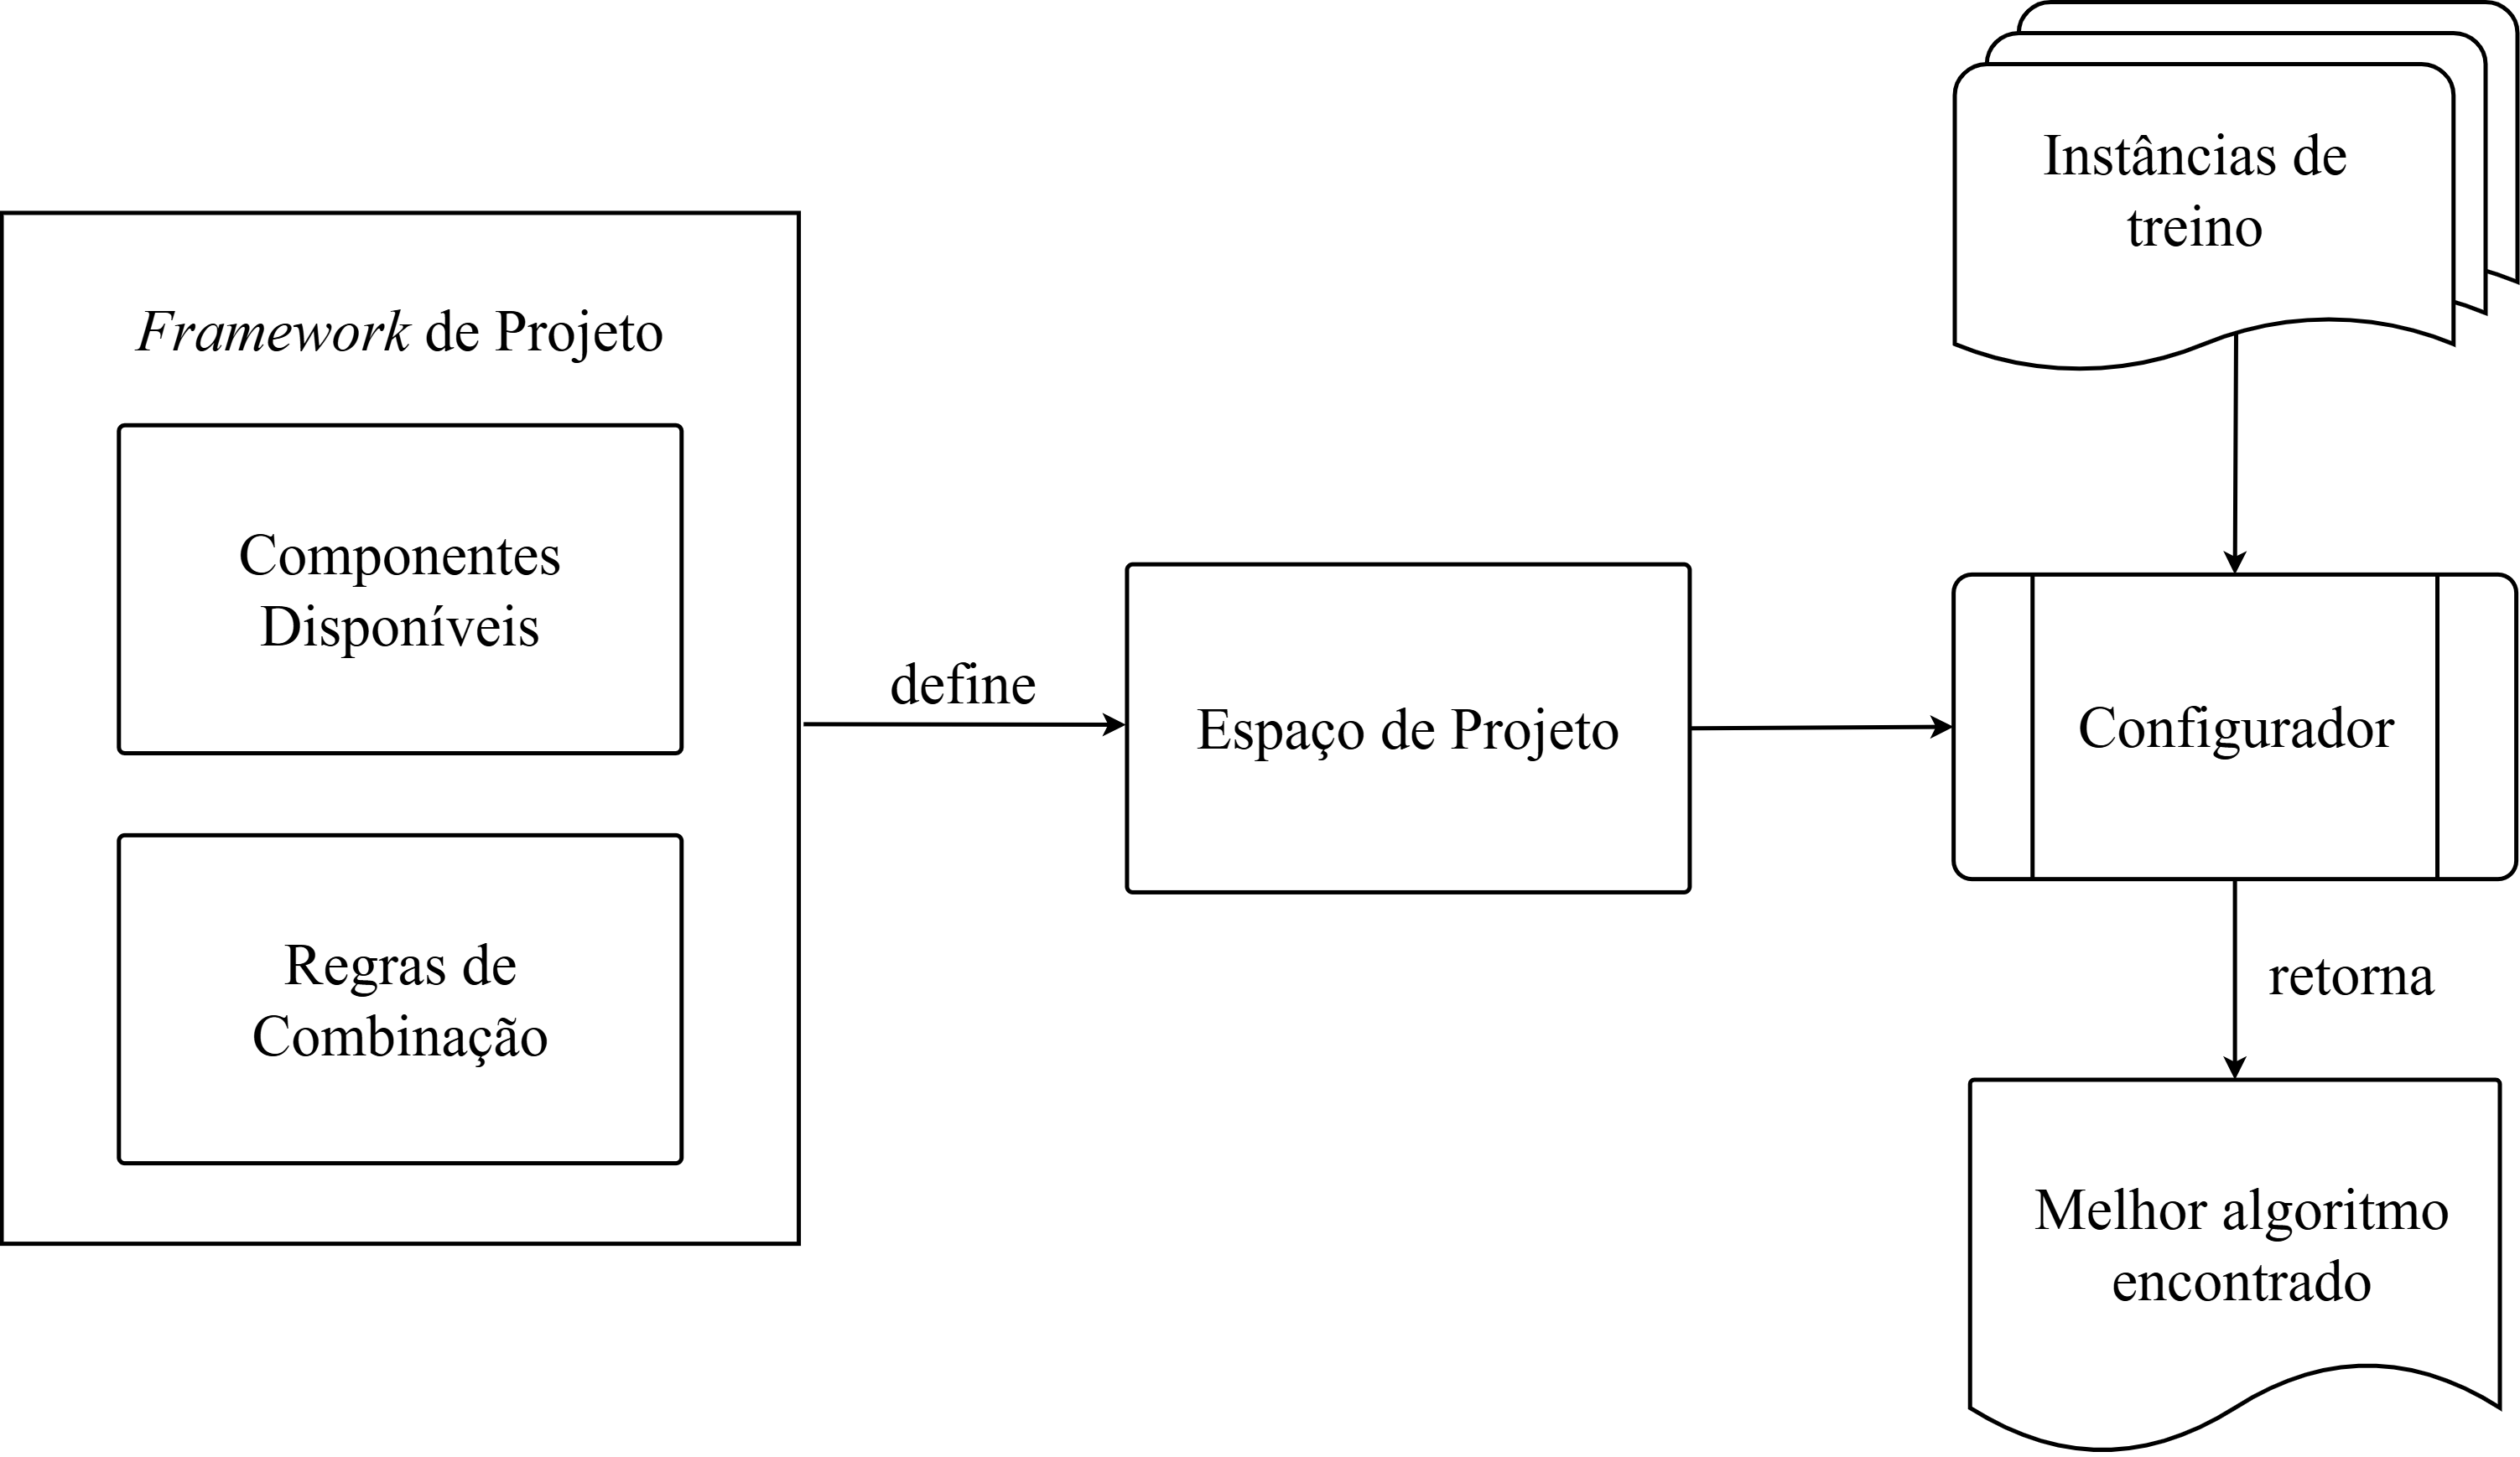
\includegraphics[width=0.60\linewidth]{img/diagrama_projeto_automatico.png}
    \caption*{\small \textbf{Fonte:} Adaptado de \cite{souza2022automatic}}
\end{figure}

\subsection{Abordagem \textit{Top-Down}}\

Uma abordagem \textit{Top-Down}, de forma geral, significa observar o problema do mais alto nível para o mais baixo. Mais especificamente, no contexto do projeto automático de algoritmos, isso significa determinar um modelo de alto nível de um algoritmo e utilizar componentes específicos para instanciar os componentes genéricos desse modelo. Nessa abordagem, o algoritmo resultante sempre terá o formato do modelo definido \citep{mascia2013grammars}. Por exemplo, podemos considerar o Algoritmo \ref{alg:ils} explicado anteriormente como nosso modelo. Recapitulando, precisamos definir quatro componentes para obter um algoritmo de \ac{ILS}: solução inicial, melhoria, perturbação e critério de aceitação. Dessa forma, independentemente de quais componentes específicos escolhermos instanciar, ao final do processo, sempre obteremos uma \ac{ILS}. A Tabela \ref{tab:estrategias_ils} reúne possibilidades de implementação para cada um dos componentes genéricos do modelo.

\begin{table}[h!]
\centering
\caption{Estratégias disponíveis para cada componente da meta-heurística ILS}
\label{tab:estrategias_ils}
\begin{tabular}{lc}
\hline
\textbf{Componente} & \textbf{Estratégias}  \\ 
\hline
Solução Inicial             & \texttt{Construtiva, Aleatória} \\ 
Melhoria                     & \texttt{Busca Tabu, Busca Local, Recozimento Simulado}   \\
Perturbação                 & \texttt{Vizinho Aleatório, Alteração Aleatória}  \\
Critério de Aceitação       & \texttt{Aceita Melhora, Aceita Qualquer, Metrópolis}   \\
\hline
\end{tabular}
    \caption*{\small \textbf{Fonte:} Os Autores.}

\end{table}

A partir da definição dessas componentes específicas, podemos instanciar diferentes algoritmos de \ac{ILS} a partir do modelo. Dessa maneira, podemos buscar as combinações de componentes mais eficientes. No processo de definição dos componentes, precisamos levar em conta que o número de componentes específicas disponíveis afeta diretamente a quantidade de algoritmos que podemos gerar. Por isso, precisamos equilibrar a variabilidade de opções com a complexidade de explorar esse espaço de configuração \citep{souza2022automatic}.

Nesse tipo de abordagem, podemos modelar as regras de combinação dos componentes como parâmetros categóricos de um algoritmo. Por exemplo, poderíamos implementar cada um dos métodos de melhoria e definir um parâmetro categórico $p_i$ que determinaria qual estratégia de melhoria o algoritmo utilizaria na execução de forma que $p_i \in \{\texttt{buscaTabu}, \texttt{buscaLocal}, \texttt{recozimentoSimulado} \}$. Além disso, certas estratégias precisam de parâmetros adicionais; por exemplo, ao instanciarmos a busca tabu como processo de busca, precisamos definir qual vizinhança utilizar e um valor para o parâmetro \textit{tenure}. Podemos modelar esses parâmetros adicionais como parâmetros numéricos ou categóricos condicionais. Dessa forma, a partir dessas ideias, podemos parametrizar as decisões de projeto de algoritmos e utilizar os configuradores já existentes para gerar algoritmos automaticamente. \citep{souza2022automatic} 

Através de trabalhos como \cite{khudabukhsh2016satenstein}, \cite{franzin2019revisiting} e \cite{ bezerra2020automatically}, podemos verificar a efetividade da abordagem \textit{Top-Down} em gerar algoritmos efetivos (veja a Seção \ref{sect:bibconfig} para mais detalhes sobre os trabalhos da literatura de \ac{AAC} e \ac{AAD}). Porém, para utilizá-la eficientemente, precisamos determinar previamente o modelo do algoritmo e considerar as possíveis interações entre cada um dos componentes implementados. Essa tarefa se torna mais difícil à medida que o número de componentes cresce \citep{mascia2014grammar}. Por esse motivo, podemos utilizar, alternativamente, a estratégia \textit{Bottom-Up} para automatizar o processo de desenvolvimento de algoritmos de forma mais flexível.

% A figura \ref{img:algoritmos_ils_instanciados} mostra dois exemplos de possíveis algoritmos \ac{ILS} gerados. Podemos observar que cada um deles utiliza combinações totalmente diferentes de componentes, de forma que eles obteriam resultados diferentes ao executar as instâncias de treinamento.

% \begin{figure}[h!] 
%     \centering
%     \caption{Possíveis algoritmos ILS gerados com a abordagem \textit{Top-Down} de projeto automático de algoritmos}
%     \label{img:algoritmos_ils_instanciados}
%     \includegraphics[width=0.85\linewidth]{img/algoritmos_ils_instanciados.png}
% \end{figure}



\subsection{Abordagem \textit{Bottom-Up}} \label{sect:bottomup}

A abordagem \textit{Bottom-Up} nos permite focar no desenvolvimento dos componentes algorítmicos sem precisarmos determinar o formato do algoritmo final. Além de simplificar algumas fases do processo, essa abordagem tende a gerar algoritmos totalmente novos e híbridos.

Apesar da flexibilidade na geração de algoritmos, ainda precisamos definir as regras de combinação dos componentes. Uma das formas de representar esse cenário é utilizando uma gramática livre de contexto na forma Backus-Naur. Definimos essa gramática de forma que qualquer derivação das regras gere um algoritmo válido \citep{mascia2013grammars}. Na Figura \ref{img:gram_backus_exemplo} podemos ver um exemplo de gramática capaz de gerar algoritmos compostos por diferentes combinações de componentes. Para a definição e teoria em gramáticas livres de contexto, veja \cite{papadimitriou1997elements}.

\begin{figure}[h!] 
    \centering
    \caption{Gramática livre de contexto na forma Backus-Naur para geração de um algoritmo de busca}
    \label{img:gram_backus_exemplo}
    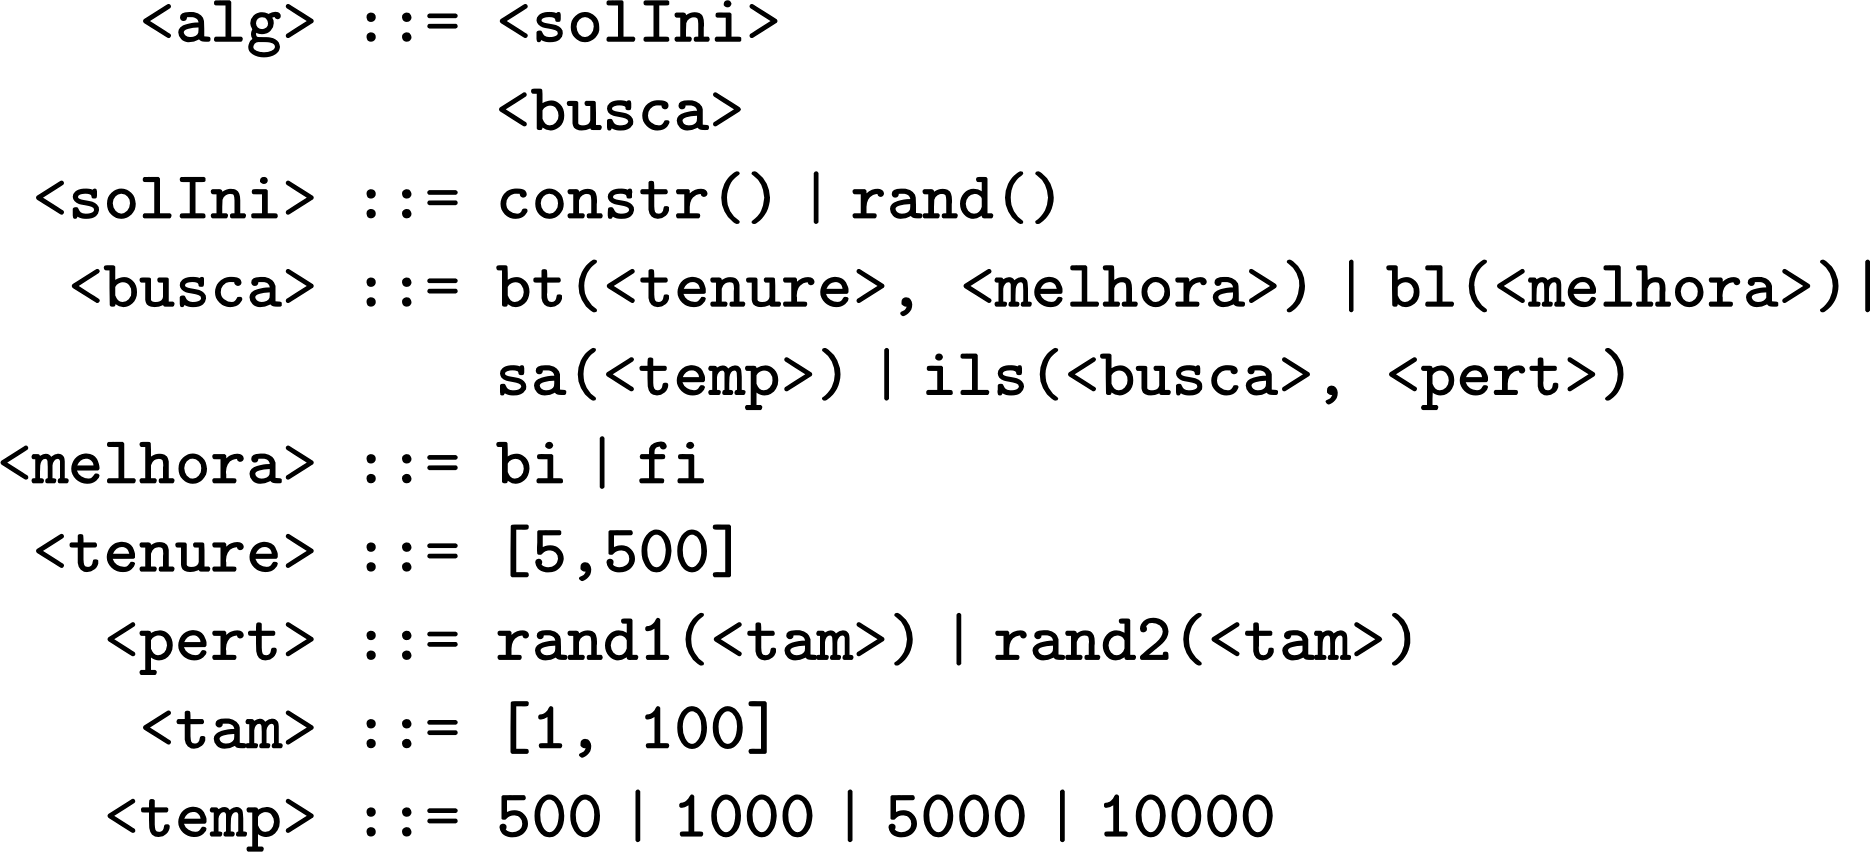
\includegraphics[width=0.75\linewidth]{img/gram_backus_exemplo.png}
    \caption*{\small \textbf{Fonte:} Os Autores.}
\end{figure}

A gramática é composta por uma série de regras de transformação de símbolos não terminais. A forma Backus-Naur representa os símbolos não terminais entre os caracteres \texttt{<>}. Cada regra define uma escolha de projeto. Por exemplo, o símbolo inicial da gramática de exemplo é o \texttt{<alg>}. Esse símbolo deriva para os não terminais de solução inicial \texttt{<solIni>} e processo de busca \texttt{<busca>}, indicando que esses componentes devem existir no algoritmo. O primeiro símbolo deriva para algumas estratégias de gerar soluções iniciais, enquanto o segundo tem o potencial de gerar métodos de busca inteiros sofisticados e híbridos. Cada um dos métodos de busca $\texttt{bt}$ (Busca Tabu), $\texttt{bl}$ (Busca Local), $\texttt{sa}$ (\textit{Simulated Annealing}) e $\texttt{ils}$ (Busca Local Iterada) possui seus próprios argumentos, os quais outros símbolos não terminais determinam; inclusive, um deles recebe outro método de busca como argumento, gerando recursividade na gramática.

Podemos notar que os símbolos não terminais da gramática derivam ou para um conjunto determinado de valores ou para um intervalo numérico específico. A partir dessa percepção, \cite{mascia2013grammars} propôs mapear os símbolos não terminais para parâmetros categóricos ou numéricos em um algoritmo e, com isso, utilizar técnicas de \ac{AAC} para realizar a derivação da gramática. Dessa forma, um símbolo não terminal que deriva de outro símbolo não terminal se torna um parâmetro condicional em relação ao parâmetro do símbolo gerador. Também precisamos tratar da recursividade da gramática, visto que um algoritmo possui um conjunto finito de parâmetros. \cite{mascia2013grammars} propõe criar cópias dos parâmetros para cada nível permitido de recursão, de forma que os parâmetros do nível $i+i$ sejam condicionais ao parâmetro que gera a recursão no nível $i$.
 

% \section{Teoria de Complexidade}é capaz 

% Entender conceitos de complexidade de algoritmos e de problemas é essencial quando se busca soluções para problemas, no sentido de que essas ferramentas permitem avaliar a viabilidade de uma solução a partir do seu consumo de tempo e espaço. Esta seção expõe formas de medir o tempo de execução de algoritmos e formas de classificar problemas pela sua complexidade inerente.

% \subsection{Complexidade de Algoritmos}

% O tempo de execução de um algoritmo em uma máquina é influenciado por diversos fatores, como sistema operacional da máquina, tarefas concorrentes na máquina, dados de entrada, linguagem de programação, bibliotecas e compilador utilizados para implementação, entre outros. Além disso, execuções de algoritmos com exatamente os mesmos parâmetros em uma mesma máquina podem levar tempos diferentes para finalizar. Por isso, existem padronizações para medir a eficiência de um algoritmo. Na maioria dos casos, essa eficiência é medida no número de passos que o algoritmo leva para resolver um problema e em função do tamanho da entrada dada ao algoritmo, ou seja, a partir do momento em que a definição da função que representa o tempo de execução do algoritmo é feita, é possível prever quanto tempo ele levaria com um novo tamanho de entrada \citep{cormen2022introduction}.

% Ainda assim, expressões que definem exatamente o tempo de execução de um algoritmo tendem a ser complexas. Por isso, é mais conveniente expressar o tempo de execução através de uma estimativa. Essa estimativa é chamada de notação assintótica e consiste em considerar apenas o termo de maior ordem da expressão, ignorando fatores constantes que afetam o tempo de execução do algoritmo. Essa abordagem estabelece um limite superior do crescimento do tempo de execução em relação ao tamanho da entrada dada ao algoritmo. Com isso, é possível expressar a complexidade de um algoritmo de forma simples, mas sem causar perda de informação que possa resultar em erros de análise e de comparação entre algoritmos \citep{sipser2013introduction}.

% A exemplo, considere que a função \(f(n) = 3n^5+7n^4+n^{1/2}\) representa o tempo de execução de um algoritmo $A$. Podemos declarar que o tempo de execução assintótico desse algoritmo é $O(n^5)$, isto é, os termos de menor ordem são descartados juntamente com os fatores constantes. Com isso, temos que, independentemente de quaisquer fatores, o tempo de execução do algoritmo $A$ tem um grau de crescimento menor ou igual a $n^5$.

% No começo do estudo de complexidade de problemas, houve certo progresso em provar que alguns problemas não podem ser resolvidos em tempo polinomial, mas, para muitos problemas fundamentais, essa questão permanece sem resposta. Por isso, além de não conhecermos algoritmos polinomiais para tais problemas, também não podemos provar que eles não existam \citep{eva2005}.

% Dessa forma, podemos introduzir o conceito de verificadores polinomiais. Um algoritmo $A$ é um verificador válido de um problema $X$ se recebe como argumentos $I$ e $c$, executa em tempo polinomial e, além disso, para todas as instâncias $I$ do problema $X$ que respondem "sim", existe um polinômio $p$ tal que existe algum certificado $c$, de forma que $|c| \leq p(|I|)$, para o qual $A$ responde "sim". Com isso, podemos definir a classe de problemas que possuem algum verificador polinomial válido. Ela é chamada de $NP$ \citep{eva2005}.

% Por exemplo, seja $X$ o problema de, dado um grafo simples $G=(V,E)$, verificar se existe um caminho hamiltoniano em $G$. Com isso, seja $A$ um algoritmo que recebe como argumentos um grafo simples como instância de $X$ e um certificado $c$ igual a uma sequência de vértices de $G$ que formam um suposto caminho hamiltoniano. O algoritmo verifica se $|c|=|V|$, verifica se todos os vértices de $G$ estão contidos em $c$ e, para cada $v_i \in c$, verifica se existe a aresta $\{v_i, v_{i+1}\}$ em $G$. Podemos verificar que o algoritmo claramente executa em tempo polinomial pois, respectivamente, cada passo descrito leva tempo $O(|V|)$, $O(|V|^2)$ e $O(|V|*|M|)$. Além disso, se $G$ possui um caminho hamiltoniano, sempre existe um certificado $c$, o próprio caminho hamiltoniano, de forma que $|c|=|V|$, que faz o verificador descrito responder "sim". Portanto, $A$ é um verificador válido para $X$ e, consequentemente, $X$ está em $NP$ como já demonstrado por \cite{garey1976complexity}.

% As definições das classes $P$ e $NP$ geram a consequência de que $P \subseteq NP$. Seja $X$ um problema qualquer da classe $P$. Ademais, seja $A$ um algoritmo polinomial que resolve $X$. Com isso, definimos o algoritmo $B$ que, dada uma instância $I$ de $X$ e um certificado $c$, utiliza o algoritmo $A$ internamente para resolver a instância $I$ e devolve a resposta de $A$ como sua resposta. Podemos verificar que, se $A$ resolve $X$, o algoritmo $B$ responde "sim" se e somente se $I$ é uma instância "sim". Além disso, o certificado $c$ não importa na verificação e, como $A$ é polinomial, $B$ também é. Portanto, podemos concluir que todos os problemas de $P$ possuem um verificador válido e, com isso, temos que $P \subseteq NP$ \citep{eva2005}.



% Outro conceito que precisamos introduzir é a redução polinomial entre dois problemas. Dados dois problemas $A$ e $B$, reduzir o problema $A$ para o problema $B$ significa definirmos uma função $f$ que mapeia todas as instâncias de $A$ para instâncias de $B$. O mapeamento deve funcionar de forma que, para qualquer instância de $A$, $I_A$, a sua imagem $f(I_A)$ responde "sim" para o problema $B$ se e somente se $I_A$ responde "sim" para o problema $A$. Em outras palavras, se uma redução de $A$ para $B$ existe, podemos utilizar um algoritmo que resolve $B$ para resolver $A$ através da redução das instâncias de $A$. Uma redução polinomial entre dois problemas $A$ e $B$, escrita $A \leq_p B$, é uma redução que pode ser computada em tempo polinomial \citep{eva2005}.

% Uma consequência da definição de redução polinomial é que se existe uma redução polinomial $A \leq_pB$ e existe um algoritmo que resolve $B$ em tempo polinomial, então $A$ também pode ser resolvido em tempo polinomial. Perceba que, dada a instância $I_A$ de $A$, basta realizar a redução que leva tempo polinomial e executar o algoritmo polinomial do problema $B$ sobre a instância $f(I_A)$. Dessa forma, a composição das duas fases polinomiais gera um algoritmo polinomial que resolve $A$.

% A definição de reduções polinomiais nos permite apresentar outra classe de problemas. Os problemas NP-Difíceis. Um problema $X$ é NP-Difícil se, para cada problema $Y$ da classe $NP$ existe uma redução polinomial $X \leq_pY$. Por conta dessa definição, caso algum pesquisador encontre um algoritmo polinomial para qualquer problema NP-Difícil, todos os problemas de NP serão resolvíveis em tempo polinomial implicando em $P=NP$.

% \section{Métodos Heurísticos(TODO:adicionar pseudocódigos de exemplo}



% Entender o funcionamento de diferentes métodos heurísticos é importante para este trabalho por dois motivos principais. Primeiramente, precisamos compreender as estratégias para que, a partir disso, possamos combiná-las utilizando técnicas de configuração automática. Ademais, visto que o objetivo das técnicas de configuração automática é automatizar a combinação de componentes heurísticos, precisamos entender as componentes para verificar o ganho proporcionado por essas técnicas. Esta seção aborda conceitos básicos de heurísticas e meta-heurísticas através da definição de vizinhança e detalhamento dos principais métodos heurísticos que serão úteis ao escopo deste trabalho.

% \subsection{Vizinhanças}

% Dado o conjunto de todas as soluções de um problema $S$, \cite{talbi} define uma vizinhança como um mapeamento de cada solução $s \in S$ para um subconjunto de soluções $N(s) \subseteq S$. Chamamos de vizinha de $s$ uma solução $s' \in N(s)$. O mapeamento da vizinhança modifica soluções sistematicamente para gerar novas soluções. Por isso, a vizinhança é uma componente específica ao problema-alvo, isto é, sua forma e eficiência dependem exclusivamente de características do problema. Isso é verdade pois modificar uma solução inclui manipular a representação da solução, representação essa que varia entre problemas e até mesmo entre diferentes abordagens sobre o mesmo problema \citep{talbi}.

% O autor de uma vizinhança deve considerar algumas características durante o desenvolvimento. Uma delas é a localidade da vizinhança; essa propriedade consiste no impacto que alterações na representação de uma solução têm sobre a qualidade da solução. Se pequenas alterações na representação causam pequenas mudanças na solução, a vizinhança possui baixa localidade. Por outro lado, se pequenas alterações na representação causam grandes mudanças na solução, a vizinhança possui alta localidade. Nesse sentido, uma exploração do espaço de busca por meio de uma vizinhança com baixa localidade é mais significativa \citep{talbi}.

% Outro ponto importante é o tamanho da vizinhança. Gerar e explorar uma vizinhança muito grande pode ter um custo muito alto e, com isso, atrapalhar o processo de busca. Por outro lado, vizinhanças muito restritas e, consequentemente, pequenas, podem ignorar soluções promissoras no espaço de soluções. \citep{talbi}.

% A partir deste ponto, precisamos introduzir uma maneira de quantificar a qualidade de uma solução chamada de função objetivo. Essa função mapeia todo o conjunto de soluções $S$ de um problema para valores reais, $f : S \to \mathbb{R}$. Essa ferramenta permite comparar soluções pela sua qualidade \citep{talbi}. Além disso, o presente trabalho trata apenas de problemas de minimização, isto é, quanto menor é o custo de uma solução, melhor é a solução. Por isso, por conveniência, em qualquer contexto, sendo $s_1$ e $s_2$ soluções para um dado problema, $f(s_1) < f(s_2)$ significará que a solução $s_1$ é melhor que a solução $s_2$.

% Com o conceito de vizinhança estabelecido, podemos introduzir o conceito de ótimo local. Esse conceito é importante pois diversas meta-heurísticas mais sofisticadas implementam múltiplas técnicas para evitar ótimos locais. \cite{talbi} define um ótimo local como uma solução $s'$ tal que não existe nenhuma solução $s''$ na vizinhança $N(s')$ que $f(s'') < f(s')$. Um ótimo global, por sua vez, além de também ser um ótimo local, é uma solução $s'$ que, para qualquer solução $s''$ do espaço de busca, $f(s') \leq f(s'')$ \citep{talbi}. A Imagem 1(TODO: FAZER GRÁFICO DE MÍNIMOS LOCAIS) apresenta um gráfico que representa os valores $f$ pelo espaço de busca e indica ótimos locais e ótimos globais.

% \subsection{Busca Local}

% A busca local é uma das meta-heurísticas mais básicas e, por isso, meta-heurísticas mais sofisticadas utilizam seus conceitos internamente. Dada uma solução inicial $s_0$, a cada iteração $i$, a busca local gera a vizinhança $N(s_i)$ da solução $s_i$. Com isso, a busca local seleciona uma solução $s_{i+1} \in N(s_i)$ tal que $f(s_{i+1}) < f(s_i)$, em outras palavras, seleciona uma solução que melhora a função objetivo. Por fim, o algoritmo finaliza o processo de busca quando não existe nenhuma solução $s' \in N(s_i)$ de forma que $f(s') < f(s_i)$. Por esse motivo, a busca local não consegue escapar de ótimos locais no espaço de busca \citep{talbi}.

% Podemos realizar a exploração do espaço de busca e a seleção de vizinhos na busca local de diferentes formas. Uma delas, a seleção por melhor melhora, consiste em selecionar o melhor vizinho de uma solução a cada iteração, isto é, tendo uma solução $s_i$, o algoritmo seleciona a vizinha de $s_i$ que oferece o máximo de melhoria na função objetivo em relação a $f(s_i)$. Utilizar esse tipo de seleção significa gerar e avaliar todos os vizinhos da solução a cada iteração. Esse processo pode ter um custo elevado em vizinhanças grandes \citep{talbi}.

% \begin{algorithm}
% \caption{Busca Local}
% \label{alg:busca_local}
% \begin{algorithmic}[1]
%     \Require
%         \State $s_0$ \Comment{Solução inicial}
%         \State $N$ \Comment{Estrutura de vizinhança}
%     \Ensure
%     \State $s \gets s_0$ \Comment{Gera uma solução inicial aleatória ou por heurística.}
%     \State $houveMelhora \gets \text{verdadeiro}$
    
%     \While{$houveMelhora$}
%         \State $houveMelhora \gets \text{falso}$
%         \State $s_{melhor\_vizinho} \gets \Call{BuscarMelhorVizinho}{N(s_{atual})}$ \Comment{Encontra o melhor vizinho na vizinhança $N(s_{atual})$.}
        
%         \If{$f(s_{melhor\_vizinho}) < f(s_{atual})$}
%             \State $s_{atual} \gets s_{melhor\_vizinho}$ \Comment{Atualiza a solução atual se o vizinho for melhor.}
%             \State $houveMelhora \gets \text{verdadeiro}$ \Comment{Sinaliza que a busca deve continuar.}
%         \EndIf
%     \EndWhile
    
%     \State \Return $s_{atual}$ \Comment{Retorna o ótimo local encontrado.}
% \end{algorithmic}
% \end{algorithm}

% Outra forma de selecionar vizinhos consiste em selecionar o primeiro vizinho de $s_i$ que melhora a função objetivo. Por isso, ao contrário da primeira opção, o algoritmo não precisa gerar e avaliar toda a vizinhança. Isso gera uma exploração do espaço de busca mais rápida; porém, corre-se o risco de que o processo ignore boas soluções simplesmente pela ordem de geração e avaliação dos vizinhos. Chamamos essa segunda estratégia de seleção por primeira melhora \citep{talbi}.

% O maior problema de uma busca local simples é a incapacidade de escapar de ótimos locais. Por esse motivo, buscas locais tendem a finalizar o processo de busca precocemente e sem realizar uma exploração satisfatória no espaço de busca \citep{talbi}. Nesse sentido, as próximas meta-heurísticas que abordaremos focam em implementar diferentes estratégias para sair de ótimos locais. 

% \subsection{Busca Tabu}

% A busca tabu é semelhante à busca local no sentido de que inicia a busca a partir de uma solução inicial $s_0$ e explora o espaço de busca iterativamente, selecionando novas soluções que melhoram a função objetivo. Porém, a busca tabu não encerra a busca ao chegar em um ótimo local no espaço de busca. Ao invés disso, a busca seleciona uma solução que piora a função objetivo para escapar do ótimo local. Nesse sentido, ela seleciona o vizinho com menor valor de função objetivo, mesmo que ele não seja melhor que a solução que o gerou \citep{talbi}.

% % Durante a exploração do espaço de soluções na busca local, a solução da iteração atual é sempre melhor que todas as soluções de iterações anteriores. Por outro lado,
% Diferentemente da busca local, a busca tabu, ao selecionar soluções que pioram a função objetivo, permite que soluções selecionadas em iterações anteriores sejam melhores que a solução da iteração atual. Por isso, é intuitivo pensar que a busca pode ficar presa em um ciclo infinito de pioras e melhoras da função objetivo. Porém, a busca tabu utiliza uma memória para evitar selecionar soluções repetidas. Ela implementa essa memória em uma lista tabu que armazena informação sobre soluções anteriormente acessadas e, com essa informação, não reexplora soluções \citep{talbi}.

% A implementação da lista tabu depende de características específicas do problema-alvo. Armazenar as soluções integralmente nem sempre é viável pelo espaço de armazenamento necessário e pelo custo de verificar se uma solução está na lista. Por isso, em certos problemas, é mais vantajoso armazenar uma informação parcial das soluções e, com isso, ganhar eficiência de verificação da lista em detrimento da precisão de verificação \citep{talbi}.
% % Por exemplo, podemos implementar a lista tabu de forma que ela armazene os movimentos que o algoritmo realizou na solução entre cada iteração e barrar novas soluções que revertam esses movimentos. Essa estratégia torna eficiente verificar se a lista tabu permite um movimento, mas não impede que o algoritmo selecione soluções repetidas, visto que, em certos problemas, é possível retornar à mesma solução por diferentes sequências de modificações \citep{talbi}.  

% \subsection{Busca Local Iterada}

% % Ao analisarmos o comportamento de uma busca local, observamos que 
% O resultado que a busca local obtém depende da solução inicial utilizada, pois cada solução inicial está associada a um número limitado de ótimos locais. Nesse sentido, a busca local iterada (ILS) realiza, iterativamente, buscas locais com diferentes soluções iniciais para encontrar diferentes ótimos locais. Porém, para realizar uma exploração mais significativa do espaço de busca, a ILS utiliza como solução inicial, em cada iteração, uma perturbação do ótimo local encontrado na iteração anterior. Dado que um ótimo local possui características de uma boa solução, pode ser mais vantajoso continuar a busca a partir dos seus vizinhos ao invés de voltar para uma solução aleatória \citep{talbi}.
% % Essa estratégia é baseada na ideia de que, sendo o ótimo local a melhor solução em uma certa área do espaço de busca, ele possui características de uma boa solução e, por isso, devemos manter algumas delas para alcançar outra boa solução \citep{talbi}.

% Algumas características da ILS incluem a possibilidade de utilizar qualquer heurística de solução única como método de busca, isto é, o processo de encontrar um ótimo local a cada iteração é uma caixa-preta para a ILS no sentido de que essa caixa-preta deve receber uma solução e encontrar um ótimo local \citep{talbi}.

% Além disso, o processo de perturbação do ótimo local é outro componente importante para a ILS. Esse procedimento tem como objetivo afastar o processo de busca dos ótimos locais encontrados em cada iteração. O impacto da perturbação na solução pode variar a depender da estratégia. Por exemplo, quando o processo de busca utilizado é altamente eficiente, realizar uma pequena modificação na solução fará com que o processo de busca encontre o mesmo ótimo local na próxima iteração, fazendo a ILS ficar presa em um ciclo \citep{talbi}.

% Por fim, após realizar a perturbação e o processo de busca sobre o ótimo local perturbado, a ILS utiliza, na próxima iteração, o novo ótimo local encontrado pela heurística de busca apenas se ele passar em um critério pré-determinado. Esse critério varia em um espectro no qual um dos extremos é aceitar apenas soluções que melhoram a função objetivo e o outro extremo é aceitar soluções independentemente de seus valores na função objetivo. Ao utilizarmos uma ILS para resolver um problema, é importante encontrarmos um ponto nesse espectro que seja adequado às particularidades do problema-alvo \citep{talbi}.

% \subsection{\textit{Variable Neighborhood Search}}

% A meta-heurística de busca em vizinhança variável (\textit{Variabel Neighborhood Search} - \ac{VNS}) se apoia na ideia de que diferentes vizinhanças de um mesmo problema exploram subespaços de busca diferentes. Nesse sentido, a estratégia consiste em explorar o espaço de busca utilizando um conjunto predefinido de diferentes vizinhanças para evitar e escapar de ótimos locais \citep{talbi}.

% Mais especificamente, podemos dividir o processo de busca na \ac{VNS} em três fases: \textit{Shake}, busca local e \textit{move}. Dada uma lista de estruturas de vizinhança $N = \{N_1, N_2,...N_{n-1}, N_n\}$, a cada iteração, a \ac{VNS} realiza o \textit{shake} de uma solução inicial $s$ pela vizinhança atual $N_k \in N$, isto é, o algoritmo seleciona uma solução $s'$ aleatoriamente da vizinhança $N_k(s)$. Após o \textit{shake}, a \ac{VNS} aplica um processo de busca local sobre a solução $s'$, encontrando um ótimo local $s''$. Por fim, caso $f(s'') < f(s)$, o \ac{VNS} realiza o \textit{move}, ou seja, seleciona $s''$ para a próxima iteração e redefine $k=1$; caso contrário, o algoritmo repete todo o processo utilizando a solução $s$ com $k = k+1$ \citep{talbi}.

% \subsection{Algoritmos Evolutivos}

% Todas as meta-heurísticas abordadas anteriormente trabalham apenas com uma solução a cada iteração, isto é, esses processos de busca observam o resto do espaço de busca a partir de uma única solução. Ao caracterizarmos estratégias por esse ponto de vista, podemos observar um outro tipo de método de busca que trabalha com um conjunto de soluções a cada momento. Chamamos esses métodos de heurísticas de população no sentido de que uma população se refere a um conjunto definido de soluções \citep{talbi}.

% Dentro da classe de heurísticas de população existem os algoritmos evolutivos. Esses métodos heurísticos se baseiam na competição entre soluções de forma a simular a evolução de espécies. Nesse sentido, também são caracterizados pela sua potencial complexidade ao serem aplicados em problemas de otimização \citep{talbi}. Esta seção não tem como objetivo detalhar todos os pormenores das técnicas utilizadas na computação evolutiva. Nesse sentido, o objetivo é estabelecer conceitos básicos que serão úteis ao entendimento de técnicas que serão posteriormente citadas.

% Algoritmos evolutivos se dividem em fases que, geralmente, são comuns a quase todas as suas subclasses. Inicialmente, o algoritmo gera uma população inicial. Tal processo é feito de forma aleatória ou por meio de alguma estratégia específica. Além disso, também temos uma função objetivo que determina a qualidade de cada solução. A partir da população gerada, o algoritmo seleciona alguns indivíduos para serem os pais das novas soluções. Os critérios de seleção podem variar, mas a estratégia mais comum é que soluções com melhor qualidade tenham maior probabilidade de serem selecionadas \citep{talbi}.

% Em seguida, o algoritmo reproduz os indivíduos selecionados de forma a gerar soluções filhas. As técnicas mais comuns para isso incluem \textit{crossover} e mutação de indivíduos. O algoritmo, então, realiza um processo de substituição para selecionar subconjuntos dos indivíduos pais e filhos para formarem a população da próxima iteração. Por fim, chamamos todo esse processo de geração e podemos vê-lo, na prática, como uma iteração de um algoritmo evolutivo \citep{talbi}.

% \section{Grafos}



% A estrutura de um grafo suporta diversas modelagens de conceitos do mundo real. Entender essa estrutura não só capacita o indivíduo a criar modelos que representam conceitos reais, mas também permite manipular e utilizar esses modelos em prol da resolução de problemas. Esta seção explica conceitos da teoria de grafos que serão úteis ao escopo deste trabalho.

% \subsection{Grafo Acíclico Direcionado}

% \subsection{Ordenação Topológica}

